\documentclass[a4paper, 11pt, oneside]{report} 
\usepackage[left=1in, right=1in, top=1in, bottom=1in]{geometry}
\newcommand{\plogo}{\fbox{$\mathcal{PL}$}} 
\usepackage{graphicx}
\graphicspath{{report_file/}{../figures/}}
\usepackage{graphics}
\usepackage{float}
\usepackage[table,xcdraw]{xcolor}
\usepackage[utf8]{inputenc} 
\usepackage[T1]{fontenc} 
\usepackage{fouriernc} 
\usepackage{subcaption}
\usepackage{tikz}
\usetikzlibrary{shapes.geometric, arrows, positioning, fit, calc, backgrounds}
\usepackage{pgfplots}
\pgfplotsset{compat=1.18}
\usepackage{graphics}
\usepackage{longtable}
\usepackage[nottoc]{tocbibind}
\usepackage{url}
\usepackage{hyperref}
\usepackage{amsmath}
\usepackage{lipsum}
\usepackage{pgfgantt} % For Gantt charts
\usepackage{pdflscape} % For landscape pages if Gantt chart is wide
\usepackage{booktabs} % For better tables
\usepackage{multirow}
\usepackage[boxed]{algorithm}
\usepackage{algpseudocode}
\usepackage[none]{hyphenat}

\begin{document} 	
    \sloppy
    \setlength{\parindent}{0em}
    \setlength{\parskip}{0.5em}
    
	\begin{titlepage} 
		
		\centering 
		
		\vspace*{\baselineskip} 
		
		\vspace{0.75\baselineskip}
		
		{\LARGE \textbf{CyberShield: Uncertainty-Aware Fraud Detection with Human-in-the-Loop Calibration for Cybercrime Intelligence}}
		
		\vspace{0.75\baselineskip}
		
		\vspace{2\baselineskip}

		A report submitted for the course named Project - I (CS3201)
		
		\vspace*{7\baselineskip}
		
		Submitted By
		
		\vspace{0.5\baselineskip}
		
		{\scshape\Large ABHISHEK YADAV \\ SEMESTER - VI \\ 230103041}
		
		\vspace{0.5\baselineskip}
		
		Supervised By
		
		\vspace{0.5\baselineskip}
		
		{\scshape\Large Dr. Salam Michael Singh}
		\vspace{0.5\baselineskip}
		
		\vfill
		
		\begin{center}
			
\includegraphics[width=5cm]{report_file/iiit manipur.png}
		\end{center}
	
	{\scshape\small Department of Computer Science and Engineering\\ Indian Institute of Information Technology Senapati, Manipur \\ April, 2026}
	
\end{titlepage}

%----------------------------------------------------------------------------------------

% \begin{center}
\begin{center}
   { \LARGE \textbf{Declaration}}
\end{center}
In this submission, I have expressed my idea in my own words, and I have adequately cited and referenced any ideas or words that were taken from another source. I also declare that I adhere to all principles of academic honesty and integrity and that I have not misrepresented or falsified any ideas, data, facts, or sources in this submission. If any violation of the above is made, I understand that the institute may take disciplinary action. Such a violation may also engender disciplinary action from the sources which were not properly cited or permission not taken when needed.

\vspace{1cm}\hspace{8.35cm} ABHISHEK YADAV \\
\vspace{1cm}\hspace{9cm} 230103041 \\

\newpage

\begin{center}
	\thispagestyle{empty}
		
		\begin{table}
			\centering
			
\includegraphics[scale=0.2]{report_file/iiit manipur.png}
			\begin{tabular}{l}
				Department of Computer Science and Engineering \\
				Indian Institute of Information Technology Senapati, Manipur \\
			\end{tabular}
		\end{table}
		\par\noindent\rule{\textwidth}{0.4pt}
			\textbf{Dr. Salam Michael Singh}
			\hspace*{\fill} Email: \href{mailto:michael_s@iiitmanipur.ac.in}{michael\_s@iiitmanipur.ac.in}\\
			Assistant Professor
			\hspace*{0pt}\hfill Contact No: +91 8575443081\\[2cm]
			{\Huge \textbf{\emph{To Whom It May Concern}}}\\[2cm]
			\linespread{1.13}
			\large{This is to certify that the project report 
                entitled \textbf{"CyberShield: Uncertainty-Aware Fraud Detection with Human-in-the-Loop Calibration for Cybercrime Intelligence",} submitted to the department of Computer Science and Engineering, Indian Institute of Information Technology Senapati, Manipur in partial fulfillment for the award of degree of Bachelor of Technology in Computer Science and Engineering is a bonafide record of work carried out by \textbf{ABHISHEK YADAV} bearing roll number 230103041.}\\[2.0cm]
			\hspace*{2.6in}\large{Signature of Supervisor}\\[0.3cm]
			\hspace*{2.5in}\textbf{(Dr. Salam Michael Singh)}\\[0.5cm]
			
	\end{center}
        \vspace{0.5cm}
	Signature of the Examiner 1 ............................\\\\
	Signature of the Examiner 2 ............................\\\\
	Signature of the Examiner 3 ............................\\\\
	Signature of the Examiner 4 ............................\\\\
	\newpage
 

\newpage
\addcontentsline{toc}{chapter}{Abstract}
\begin{center}
    { \LARGE \textbf{Abstract}}
\end{center}
\vspace{2cm}
{\large
Cybercrime via SMS, WhatsApp, and URLs represents a rapidly escalating threat necessitating robust automated detection. Conventional machine learning approaches often suffer from poor calibration and high false-positive rates. In this report, we present \textbf{CyberShield}, an uncertainty-aware fraud detection framework utilizing a calibrated ensemble model (Logistic Regression, SVM, and Naive Bayes) on high-dimensional TF-IDF vectors. The system employs confidence-bounded thresholding: highly certain malicious patterns \linebreak ($P(Fraud) \geq 0.90$) trigger automated generation of a pre-filled NCRP-compliant PDF document ready for manual portal submission, while ambiguous cases \linebreak ($0.30 \leq P(Fraud) < 0.70$) are routed to an administrator panel for Human-in-the-Loop (HITL) annotation. The model is continuously adaptable through a novel \textit{False-Positive-Driven} Hard Negative Mining strategy that selectively mines the top 15\% highest-confidence False Positives and retrains with elevated sample weights ($w=2.0$), improving precision while preserving recall. Extensive evaluation on 26,534 labeled samples demonstrates a test-set accuracy of \textbf{94.87\%} and an ROC-AUC of \textbf{0.9895}. By integrating a Velocity Intelligence tracker for malicious artifacts, CyberShield provides an end-to-end, highly reproducible approach to mitigating sociotechnical cyber-attacks.
}

\newpage
        \begin{center}
            { \LARGE \textbf{Acknowledgement}}
        \end{center}
	\vspace{2cm}
	I would like to express my deepest appreciation to all those who provided me the possibility to complete this project. A special gratitude I give to my supervisor, \textbf{Dr. Salam Michael Singh}, whose contribution in stimulating suggestions and encouragement helped me to coordinate my project especially in writing this report.

	I would also like to express my sincere gratitude to the Head of the Department (CSE), \textbf{Dr. Navanth Saharia}, for his constant support and for providing the necessary facilities to successfully execute this project.
	
	Furthermore, I would also like to acknowledge with much appreciation the crucial role of the faculty and staff of the Department of Computer Science and Engineering, Indian Institute of Information Technology Senapati, Manipur, who gave the permission to use all required equipment and necessary materials to complete the tasks. 
	
	Last but not least, many thanks go to my family and friends whose support, guidance, and encouragement have been invaluable throughout this endeavor.
	
	\vspace{1cm}
	\begin{flushright}
	    \textbf{ABHISHEK YADAV} \\
	    Roll No: 230103041
	\end{flushright}
	
	\vspace{1cm}
	
	\addcontentsline{toc}{chapter}{Acknowledgement}
	\tableofcontents
	\listoffigures
        \listoftables
	\chapter{Introduction}
	\section{Background}
In the modern digital era, the proliferation of real-time communication mediums---such as Short Message Service (SMS), WhatsApp, and email---has fundamentally transformed global interconnectedness. While these platforms have brought unprecedented convenience to billions of users, they have simultaneously created an expansive attack surface for malicious actors. Cybercrime, specifically functionally motivated digital fraud, has seen a rapid rise globally. According to the FBI Internet Crime Complaint Center (IC3) 2023 Annual Report \cite{ic3_2023}, billions of dollars are lost annually to sociotechnical cyber-attacks, ranging from phishing, smishing (SMS phishing), and vishing (voice phishing) to advanced fee scams, lottery frauds, and impersonation of government authorities or financial institutions.

Traditional spam filters, built heavily on static blacklists and rudimentary regular expression targeting, have notable limitations. For instance, attackers frequently rotate malicious domains every 48 hours to evade static signature detection, rendering blacklists obsolete almost immediately. Cybercriminals employ sophisticated evasion tactics involving character obfuscation, link shortening services, and highly persuasive semantic phrasing designed to elicit an urgent emotional response from the victim. These attacks exploit human vulnerability rather than system vulnerability. Therefore, identifying these threats requires a deep contextual understanding of natural language, recognizing subtle patterns of urgency, financial requests, and implicit threats that characterize fraudulent communication.

Furthermore, the scale of legitimate communication is so vast that any automated system deployed to filter fraud must maintain a high precision rate to avoid ``alert fatigue" and the consequence of suppressing time-critical, legitimate messages (such as legitimate banking alerts or emergency communications). This balance between the false positive rate (FPR) and the true positive rate (TPR) necessitates a paradigm shift from deterministic to probabilistic, uncertainty-aware computational models. 

\section{Motivation}
The primary motivation for this project stems from the socioeconomic impact of digital fraud on demographics with lower digital literacy. Attackers frequently utilize local dialects, persuasive psychological triggers, and spoofed authoritative entities (such as banks or government agencies) to bypass the user's critical thinking. When victims do recognize they have been scammed, the reporting process is often fragmented. In India, for example, the National Cybercrime Reporting Portal (NCRP) provides a centralized mechanism for citizens to report cybercrimes. This is particularly relevant in regions like Manipur and Northeast India, where digital penetration is accelerating rapidly, yet dedicated local cyber-literacy resources remain scarce, making an automated reporting assistant valuable for the local populace. However, citizens are often unsure \textit{how} to categorize the crime, \textit{what} evidence to preserve, and \textit{where} to find the malicious indicators of compromise (IoCs) within the text payload.

There is a significant gap between the detection of a threat and the actionable intelligence required to report and mitigate it. Standard machine learning models classify text into binary buckets (Fraud vs. Legit). However, the real world operates in a continuum of uncertainty. If an AI system encounters a message it has never seen before, forcing a binary classification often leads to erratic predictions. 

This context necessitates an intelligent system capable of not only deciphering fraudulent semantics but also acknowledging its own uncertainty. A system that can confidently flag:

\begin{quote}
    \textit{"I am 40\% sure this is fraud; I require human expert review before deciding."}
\end{quote}

represents a safer, calibrated approach to real-world deployment. Consequently, the motivation is to bridge the gap between opaque AI predictions and actionable cyber intelligence by incorporating a Human-in-the-Loop (HITL) calibration and integrating directly with national reporting standards.

\section{Problem Definition}
The core problem addressed in this project is the lack of adaptive, uncertainty-aware, and actionable fraud detection systems for short-text communications. Existing solutions are predominantly binary, lack explainability for non-technical users, and do not provide an end-to-end mechanism for threat reporting.

Specifically, the problem encompasses the following sub-challenges:
\begin{enumerate}
    \item \textbf{High False Positives on Ambiguous Text:} Traditional Natural Language Processing (NLP) classifiers often misclassify borderline legitimate messages that contain financial keywords but lack fraudulent intent.
    \item \textbf{Concept Drift in Threat Vectors:} Cybercriminals continually alter their phrasing to evade detection models. Static models degrade over time without continuous, curated retraining.
    \item \textbf{Lack of Explainability:} When an AI flags a message as fraudulent, the user is rarely told \textit{why}, decreasing trust in the system. Without explainability, victims cannot identify which part of a message was suspicious, leaving them vulnerable to identical subsequent attacks.
    \item \textbf{Fragmented Reporting Workflows:} Once a threat is identified, users lack automated tools to extract the indicators of compromise (IoCs) and format them into an actionable legal complaint.
\end{enumerate}

\section{Project Objectives}
To address the aforementioned challenges, this project, titled \textbf{``CyberShield"}, aims to design, develop, and deploy a holistic machine-learning-driven cyber intelligence platform. The main objectives are:

\begin{itemize}
    \item \textbf{Uncertainty-Aware Classification:} To develop a probabilistic machine learning ensemble (combining Logistic Regression, Support Vector Machines, and Naive Bayes) that classifies text across multiple threshold-bounded risk strata (FRAUD, SUSPICIOUS, UNCERTAIN, and LEGIT) rather than forced binary outcomes (See Chapter 4.3).
    \item \textbf{Human-in-the-Loop Calibration:} To implement an administrative intelligence portal where \textit{UNCERTAIN} predictions ($0.30 \leq P(Fraud) < 0.70$) are routed for manual review. This human feedback must trigger a hard-negative mining retraining pipeline to continually calibrate the model against new threats (See Chapter 4.5).
    \item \textbf{Token-Level Explainability:} To engineer a Word Risk Heatmap that visually highlights the specific semantic tokens (words) responsible for the fraud prediction, mapped by their respective coefficient weights in the trained model (See Chapter 5.5).
    \item \textbf{Velocity Intelligence Tracking:} To build a real-time tracking database that extracts and monitors repeating malicious entities (Phone Numbers and URLs) across multiple user submissions, assigning threat levels based on frequency velocity (See Section~4.6.3).
    \item \textbf{Automated NCRP Adjudication:} To provide a one-click automated generation of an NCRP-compliant PDF report, extracting all relevant indicators of compromise (IoCs) and producing a ready-to-submit document for the victim (not a direct API submission to the portal, which is identified as a near-term future enhancement) (See Section~5.5).
\end{itemize}

\section{Scope of the Project}
The scope of CyberShield is confined to textual analysis of digital communications (SMS, WhatsApp text, Email bodies) primarily in the English language. The system is optimized for English and Romanized Hinglish text. Native script inputs in Devanagari, Meitei Mayek, or other regional scripts are outside the current scope and identified as future work (See Chapter 7.3). The system extracts specific threat vectors, namely suspicious URLs and phone numbers. 

The machine learning pipeline is bounded by the current supervised dataset of 26,534 messages. The architecture supports continuous expansion through its dynamic retraining pipeline, which can ingest new HITL-labeled samples in subsequent training cycles without requiring re-engineering. The project does not currently cover deep-packet inspection of network traffic, audio deepfake detection (vishing), or image-based steganography fraud. The user interface assumes deployment as a responsive web application optimized for both desktop and mobile access, facilitating easy copy-pasting of suspicious texts by end-users.

\section{Project Timeline and Gantt Chart}
The development of CyberShield was structured iteratively over several months, adopting an iterative, sprint-based development approach. The timeline below outlines the distinct phases from requirement gathering to final evaluation and documentation spanning from late January to mid-April 2026.

\begin{figure}[H]
    \centering
    \resizebox{\textwidth}{!}{%
    \begin{ganttchart}[
        hgrid={draw=gray!30},
        vgrid={draw=gray!20},
        x unit=0.9cm,
        y unit title=0.7cm,
        y unit chart=0.6cm,
        title/.style={fill=gray!85, draw=black, text=white},
        title label font=\small\bfseries,
        title left shift=0,
        title right shift=0,
        bar label font=\small,
        bar height=0.55,
        bar top shift=0.225,
        group label font=\small\bfseries,
        group right shift=0,
        group top shift=0.2,
        group height=0.5,
        group peaks height=0.2,
        milestone/.append style={fill=orange, draw=orange!80!black, xscale=0.6},
        link/.style={->, thick, draw=gray!60}
    ]{1}{12}
        % ── Title Row ─────────────────────────────────────────
        \gantttitle{\textbf{Project Timeline (Weeks 1--12, Jan--Apr 2026)}}{12} \\
        \gantttitlelist{1,...,12}{1} \\

        % ── Phase 1: Research — Blue ──────────────────────────
        \ganttgroup[
            group/.append style={fill=blue!70!black, draw=blue!80!black}
        ]{\textcolor{white}{\textbf{Phase 1: Research}}}{1}{2} \\
        \ganttbar[
            bar/.append style={fill=blue!45, draw=blue!70!black}
        ]{Literature Survey}{1}{2} \\

        % ── Phase 2: ML Pipeline — Teal ───────────────────────
        \ganttgroup[
            group/.append style={fill=teal!70!black, draw=teal!80!black}
        ]{\textcolor{white}{\textbf{Phase 2: ML Pipeline}}}{2}{5} \\
        \ganttbar[
            bar/.append style={fill=teal!40, draw=teal!70!black}
        ]{Data Cleaning}{2}{3} \\
        \ganttbar[
            bar/.append style={fill=teal!40, draw=teal!70!black}
        ]{Model Training}{3}{5} \\

        % ── Phase 3: Architecture — Orange ────────────────────
        \ganttgroup[
            group/.append style={fill=orange!80!red!80, draw=orange!80!black}
        ]{\textcolor{white}{\textbf{Phase 3: Architecture}}}{4}{6} \\
        \ganttbar[
            bar/.append style={fill=orange!40, draw=orange!70!black}
        ]{Ensemble Logic}{4}{5} \\
        \ganttbar[
            bar/.append style={fill=orange!40, draw=orange!70!black}
        ]{Database Design}{5}{6} \\

        % ── Phase 4: Web Application — Purple ─────────────────
        \ganttgroup[
            group/.append style={fill=violet!65!black, draw=violet!80!black}
        ]{\textcolor{white}{\textbf{Phase 4: Web Application}}}{6}{9} \\
        \ganttbar[
            bar/.append style={fill=violet!35, draw=violet!70!black}
        ]{Flask \& UI}{6}{8} \\
        \ganttbar[
            bar/.append style={fill=violet!35, draw=violet!70!black}
        ]{PDF \& Admin Panel}{8}{9} \\

        % ── Phase 5: Evaluation — Red ─────────────────────────
        \ganttgroup[
            group/.append style={fill=red!65!black, draw=red!80!black}
        ]{\textcolor{white}{\textbf{Phase 5: Evaluation}}}{9}{12} \\
        \ganttbar[
            bar/.append style={fill=red!35, draw=red!70!black}
        ]{Testing \& Bug Fixes}{9}{11} \\
        \ganttbar[
            bar/.append style={fill=red!35, draw=red!70!black}
        ]{Documentation}{10}{12}
    \end{ganttchart}%
    }
    \caption{CyberShield Project Development Timeline (Jan--Apr 2026) across 12 weekly sprints. Each phase is color-coded: Research (blue), ML Pipeline (teal), Architecture (orange), Web Application (purple), Evaluation (red).}
    \label{fig:gantt}
\end{figure}

The phased approach ensured that the core machine learning components were validated before integration into the Flask web application. Each phase concluded with a checkpoint review confirming that probability arrays passed correctly between the offline training pipeline and the online inference server.

        \chapter{Literature Survey}
        \section{Overview}
The rapid proliferation of digital communication channels has been matched by an equally rapid evolution in cybercrime methodologies. Traditional approaches to identifying unsolicited, malicious, or fraudulent electronic messages have transitioned from rudimentary rule-based filtering to sophisticated, high-dimensional machine learning frameworks. This chapter reviews the state-of-the-art literature relevant to the foundational pillars of the CyberShield project: Short Message Service (SMS) and text-based fraud detection, threshold uncertainty and active learning, and the integration of Human-in-the-Loop (HITL) methodologies in cybersecurity. This chapter is organized into four sections: classical ML approaches to spam detection (Section 2.2), NLP tooling (Section 2.3), Human-in-the-Loop and active learning paradigms (Section 2.4), and a gap analysis situating CyberShield within the existing literature (Section 2.5).

\section{Machine Learning in Spam and Fraud Detection}
The academic investigation into automated filtering of electronic messages conceptually began with email spam. However, due to the constrained character limits, informal syntactic structures, and specific colloquialisms prevalent in SMS and instant messaging platforms (like WhatsApp), traditional email detection algorithms perform poorly when directly transposed to short-text environments.

\subsection{Evolution of Text Vectorization and Modeling}
Almeida et al.~\cite{almeida2011contributions} introduced the SMS Spam Collection v.1, which remains one of the most widely used public benchmarks for SMS spam classification research. Their comparative study of standard algorithms - including Support Vector Machines (SVM) and Naive Bayes (NB) - established that Term Frequency–Inverse Document Frequency (TF-IDF) vectorization combined with linear classifiers produces competitive baseline metrics on short-text data. Subsequent work has demonstrated that adversarial obfuscation techniques (character substitution, homoglyph attacks, whitespace manipulation) can degrade detector performance, motivating the need for character-level features and dynamic retraining pipelines such as those employed in CyberShield.

Building upon this, Abid et al. \cite{abid2022spam} conducted a comprehensive comparative analysis of traditional machine learning against deep learning methodologies for SMS spam detection. Their research demonstrated that while Deep Learning models (like LSTMs and CNNs) achieve modest performance gains on highly complex, non-linear linguistic structures, traditional algorithms (specifically optimized SVM and Logistic Regression models) provide significantly faster inference times and lower computational overhead, making them well-suited for real-time deployment. Furthermore, tree-based and linear models provide inherent feature explainability, which is a critical requirement in forensic cybercrime investigations.

Similarly, Roy et al. \cite{roy2020deep} investigated deep learning mechanisms but emphasized the importance of extensive dataset curation. Their findings underscored the ``garbage in, garbage out" paradigm; highly imbalanced datasets result in models that collapse towards the majority class (typically legitimate messages). Consequently, optimal detection relies heavily on synthetic minority oversampling (SMOTE) or hard negative mining to penalize the misclassification of edge-case fraud vectors.

\subsection{Smishing and Phishing URL Detection}
A significant subset of text-based cybercrime relies on delivering malicious payloads via Uniform Resource Locators (URLs), broadly categorized as Smishing (SMS Phishing). Jain and Gupta \cite{jain2021smishing} proposed an integrated machine learning approach that does not solely rely on the semantic text of the message, but actively parses the embedded URLs to extract lexical features (e.g., URL length, presence of hyphens, highly entropic subdomains). Their work demonstrated that combining NLP semantic analysis with lexical URL analysis reduces the false positive rate.

Further solidifying this, Sahingoz et al. \cite{sahingoz2019machine} demonstrated that lexical URL features alone - domain length, character entropy, presence of suspicious tokens - can achieve over 97\% phishing detection accuracy on large-scale datasets. The consensus across multiple reviewed studies indicates that attackers frequently exploit URL shortening services (e.g., bit.ly, tinyurl) to obfuscate malicious domains from localized text scanners. To counter this, CyberShield incorporates a Velocity Intelligence module specifically designed to track the submission frequency of these shortened artifacts, flagging them as malicious based on submission volume regardless of the domain's reputation at the time of submission.

\section{Natural Language Processing Tooling}
The implementation of machine learning models requires robust frameworks capable of transforming raw, unstructured text into mathematical representations. The Natural Language Toolkit (NLTK) established the academic standard for programmatic linguistics. Their comprehensive documentation covers the necessity of stop-word removal, stemming, and lemmatization to reduce the dimensionality of the vector space, ensuring that algorithms are not distracted by syntactically necessary but semantically hollow conjugations.

Although contextual embedding approaches such as Word2Vec and BERT offer richer semantic representations, two practical constraints favored TF-IDF for this deployment: (i) the inference latency budget of 500ms per request, which contextual transformer models exceed on CPU-only infrastructure, and (ii) the requirement for token-level explainability via inspectable model coefficients, which is straightforward for linear models over TF-IDF features but opaque for transformer embeddings. For the predictive modeling phase, the \textit{scikit-learn} library has become the de facto standard in the machine learning community. Their architecture provides standardized, interchangeable modules for vectorization, enabling researchers to rapidly prototype ensemble mechanisms. CyberShield utilizes these exact theoretical mathematical constructs to perform its soft-voting probability aggregation.

\section{Human-in-the-Loop (HITL) and Active Learning}
A glaring deficiency in modern commercial fraud filters is their deterministic binary nature. Models are mathematically forced to classify a message as $1$ (Fraud) or $0$ (Legit), often making arbitrary decisions on messages that sit squarely on the algorithmic decision boundary. 

\subsection{The Necessity of the Human Operator}
Holzinger \cite{holzinger2016interactive} explored this paradox extensively in the context of health informatics, positing the question: \textit{When do we need the human-in-the-loop?} Holzinger argues that in domains where the cost of a false positive is catastrophic, fully autonomous ``black-box" AI is suboptimal. Instead, algorithms should be utilized to perform the heavy lifting of parsing vast datasets, extracting the ambiguous ``uncertain" samples, and presenting them to a human expert. The human leverages contextual domain knowledge that the AI lacks, annotates the ambiguous sample, and feeds it back into the training loop. This specific philosophy explicitly underpins CyberShield's multi-tier thresholding logic, where probabilities between $0.30$ and $0.70$ are deferred to admin authorities rather than guessed autonomously.

\subsection{Concept Drift and Active Learning Paradigms}
This mechanism of querying a human expert is formally known in academic literature as Active Learning. Settles \cite{settles2009active} provides the definitive survey on Active Learning, outlining various query strategies. The most relevant to threat intelligence is ``Uncertainty Sampling," where the model queries the human operator for the labels of instances about which it is least certain. Furthermore, active learning directly mitigates the phenomenon of \textit{Concept Drift} \cite{gama2014survey}, where the statistical properties of the target variable (e.g., spam patterns) change rapidly over time. Settles shows that selecting boundary cases for human labelling enables a machine learning model to reach a target accuracy with substantially fewer labelled instances than random passive sampling.

\subsection{Hard Negative Mining}
Addressing class imbalance and boundary ambiguity programmatically leads to the concept of Hard Negative Mining. Shrivastava, Gupta, and Girshick \cite{shrivastava2016training} presented an online hard example mining algorithm initially designed for region-based object detectors in computer vision. While originating in computer vision, the core principle of heavily penalizing high-confidence errors transfers directly across domains and is highly effective when adapted for NLP fraud detection. In the context of CyberShield, a ``hard negative" is a highly suspicious legitimate message (e.g., an urgent banking OTP) that the model incorrectly flags as a scam. By programmatically extracting these failures during the cross-validation phase and forcing the model to retrain explicitly on them, the decision boundary is shifted away from the legitimate class distribution, reducing the risk of false alarms on borderline cases.

\section{Gap Analysis and CyberShield Contribution}
The reviewed literature reveals a significant disconnect between theoretical machine learning accuracy and practical, real-world deployment in cybercrime mitigation. Most studies conclude upon achieving a marginally superior accuracy metric on static, sterile datasets. 

There is a notable gap in literature regarding end-to-end socio-technical pipelines. Academic models do not translate their raw probabilistic outputs into actionable intelligence for the victim (such as an automated NCRP FIR schema). Furthermore, public datasets suffer from extreme temporal decay; a model trained predominantly on 2011-era SMS spam vectors (such as the Almeida dataset~\cite{almeida2011contributions}) is likely to underperform against contemporary WhatsApp KYC and PAN-card update scams that did not exist when the dataset was compiled. 

CyberShield addresses this gap by combining the established robustness of TF-IDF ensemble modelling with Holzinger's Human-in-the-Loop paradigm~\cite{holzinger2016interactive} and iterative Hard Negative Mining~\cite{shrivastava2016training}. The result is an auto-calibrating fraud detection platform that integrates with national cybercrime reporting standards rather than producing only research-grade metrics.

\subsection{Comparison with Recent Systems}
To definitively contextualize the novelty of CyberShield, Table \ref{tab:lit_comparison} illustrates a direct architectural comparison between recent notable academic systems and our proposed architecture.

\begin{table}[H]
    \centering
    \resizebox{\textwidth}{!}{
    \begin{tabular}{|l|l|c|c|c|p{5cm}|}
    \hline
    \textbf{System / Authors} & \textbf{Algorithm Core} & \textbf{Artifact Neutralization} & \textbf{HITL Calibration} & \textbf{Uncertainty Handling} & \textbf{Primary Limitation / Gap} \tabularnewline \hline
    Almeida et al. (2011) \cite{almeida2011contributions} & SVM, Naive Bayes & No & No & None & \raggedright Binary only; high false positive rate on edge cases. \tabularnewline \hline
    Roy et al. (2020) \cite{roy2020deep} & CNN / LSTM & No & No & None & \raggedright Computationally heavy; lacks explainability for cyber intelligence. \tabularnewline \hline
    Jain \& Gupta (2021) \cite{jain2021smishing} & Lexical URL + NLP & Yes (URLs only) & No & None & \raggedright Does not extract Phone Numbers; no feedback loop for concept drift. \tabularnewline \hline
    Abid et al. (2022) \cite{abid2022spam} & Optimized LR / SVM & No & No & None & \raggedright Black-box predictions without automated legal reporting integration. \tabularnewline \hline
    \textbf{CyberShield (Current)} & \textbf{Ensemble (LR+SVM+NB)} & \textbf{Yes (URLs + Phones)} & \textbf{Yes (Active Learning)} & \textbf{4-tier Probabilistic} & \raggedright \textbf{Currently English/Hinglish only; no native multilingual support.} \tabularnewline \hline
    \end{tabular}
    }
    \caption{Architectural Comparison of CyberShield against contemporary spam detection systems.}
    \label{tab:lit_comparison}
\end{table}

        \chapter{Requirement Engineering}
        \section{Introduction}
Requirement Engineering is the foundational phase of the software development lifecycle, encompassing the systematic process of gathering, analyzing, documenting, and validating the specifications of the proposed system. For the CyberShield portal, requirements are bifurcated into requirements dealing directly with the machine learning inference pipeline (backend intelligence) and those concerning the interaction logic of the front-end user interfaces (both citizen-facing and admin-facing). Functional requirements define what the system must do; non-functional requirements define how well it must do it.

\section{System Analysis}
\subsection{Limitations of the Existing System}
Before designing CyberShield, a thorough analysis of existing generic spam filters and cybercrime complaint mechanisms was conducted. The primary limitations identified were:
\begin{enumerate}
    \item \textbf{Binary Rigidity:} Existing text classifiers typically enforce a hard binary output. Messages that are highly ambiguous are frequently misclassified, offering no gradient of risk or uncertainty.
    \item \textbf{Opaque Decision Making:} Currently, when an email provider routes a message to the "Spam" folder, the user is not informed \textit{why}. This black-box approach breeds user distrust, particularly when false positives occur.
    \item \textbf{Manual Intelligence Gathering:} Victims of cybercrime must manually copy phone numbers, isolate URLs, and draft complaints from scratch when filing a First Information Report (FIR) on the NCRP portal, a process prone to transcription errors and incomplete artifact capture.
    \item \textbf{Static Models:} Most commercial off-the-shelf classifiers employ models that decay rapidly. Retraining these models requires extensive data engineering rather than a streamlined Human-in-the-Loop pipeline. Furthermore, retraining cycles in commercial systems are typically quarterly or annual, whereas cybercrime phrasing evolves on a daily basis.
\end{enumerate}

\subsection{Feasibility Study}
The feasibility of developing CyberShield was evaluated across three dimensions:
\begin{itemize}
    \item \textbf{Technical Feasibility:} The implementation of TF-IDF vectorization and classical ensemble modeling (SVM/LR/NB) on a corpus of 26,500 messages is technically feasible with low computational overhead. The system can easily be hosted on standard cloud infrastructure (e.g., Render, Heroku) using a Python/Flask ecosystem. Thus, the project is technically highly feasible.
    \item \textbf{Operational Feasibility:} By designing an intuitive citizen-facing interface and an OAuth 2.0 secured Admin panel for HITL adjudication, the system aligns perfectly with the operational workflows of civilian users and cyber-intelligence officers.
    \item \textbf{Economic Feasibility:} As the project relies entirely on open-source libraries (scikit-learn, ReportLab, Flask) and lightweight SQLite databases, capital expenditure is minimized to server hosting costs alone. Estimated monthly hosting cost on platforms such as Render or Railway is approximately USD 0--7, making the system highly cost-effective for institutional deployment.
\end{itemize}


\section{System Requirements}

\subsection{Hardware Requirements}
For deployment and continuous active retraining (Hard Negative Mining), the server infrastructure requires specific minimum capabilities to ensure the $25,000$-feature TF-IDF matrix can be processed within RAM without triggering swap space bottlenecks.
\begin{itemize}
    \item \textbf{Minimum Client Device (End User):}
    \begin{itemize}
        \item Any device with a modern browser (Chrome 90+, Firefox 88+, Safari 14+).
        \item Minimum 1Mbps internet connection.
        \item No local computation required --- all inference is server-side.
    \end{itemize}
    \item \textbf{Development Environment:}
    \begin{itemize}
        \item \textbf{Processor:} Minimum Intel Core i5 or AMD Ryzen 5 (multi-threading heavily utilized during cross-validation).
        \item \textbf{RAM:} 8 GB minimum; 16 GB recommended for manipulating the 100MB+ master dataset arrays during vectorization.
        \item \textbf{Storage:} 256 GB SSD for fast I/O read/write operations during model pickling operations.
    \end{itemize}
    \item \textbf{Production Server (Minimum):}
    \begin{itemize}
        \item \textbf{CPU:} 2 virtual Cores (vCPU).
        \item \textbf{RAM:} 1 GB (Model inferences are lightweight, taking $<100ms$).
        \item \textbf{Storage:} 20 GB block storage.
    \end{itemize}
\end{itemize}

\subsection{Software Requirements}
The software stack is uniformly Pythonic, minimizing impedance mismatch between the data science layer and the web server layer.
\begin{itemize}
    \item \textbf{Operating System:} Agnostic (Windows 11 during development; Linux/Ubuntu for deployment).
    \item \textbf{Programming Language:} Python 3.10+ is required specifically for structural pattern matching and improved dictionary ordering used in the threshold routing logic.
    \item \textbf{Machine Learning Layer:}
    \begin{itemize}
        \item \texttt{scikit-learn}: Core algorithm implementations (SVM, Logistic Regression, Naive Bayes, TF-IDF).
        \item \texttt{pandas / numpy}: Vectorized data frame manipulation and array operations (used exclusively in the offline \texttt{pipefinal.py} training pipeline, not in the runtime web server).
        \item \texttt{joblib}: Fast disk-caching and efficient binary serialization of trained model objects.
    \end{itemize}
    \item \textbf{Web Framework \& Backend:}
    \begin{itemize}
        \item \texttt{Flask}: Micro-framework handling HTTP routing and Jinja2 templating.
        \item \texttt{flask-dance}: Implementation of secure Google OAuth 2.0 authentication.
    \end{itemize}
    \item \textbf{Database \& Session Layer:}
    \begin{itemize}
        \item \texttt{Flask-SQLAlchemy} \& \texttt{psycopg2-binary}: ORM mapping and thread-safe database connection pooling.
        \item \texttt{Flask-Migrate}: Handling database schema migrations.
        \item \texttt{Flask-Login}: User session management.
    \end{itemize}
    \item \textbf{Artifact Generation:}
    \begin{itemize}
        \item \texttt{ReportLab}: Programmatic generation of the NCRP-compliant PDF utilizing Canvas draw operations.
    \end{itemize}
\end{itemize}


\section{Functional Requirements}
Functional requirements define the core behavior, inputs, outputs, and specific computational tasks the system must perform.
\begin{enumerate}
    \item \textbf{Message Ingestion \& Parsing:} The system must permit users to paste text up to 800 characters (enforced at the HTML frontend layer via the \texttt{maxlength} attribute, not the server-side backend) and systematically strip whitespace and non-printable characters.
    \item \textbf{Artifact Extraction:} The system must execute RegEx pipelines to extract and isolate all URLs (http/https/www) and 10+ digit numerical vectors resembling phone numbers.
    \item \textbf{Probabilistic Scoring:} The system must compute a soft-voting probability matrix against the text string using ensemble weights determined via grid search over the validation set, with the empirically optimal values for the current training run being (SVM=0.50, LR=0.20, NB=0.30) and classify it into bounds: 
    \begin{itemize}
        \item FRAUD: $P(\text{Fraud}) \geq 0.90$
        \item SUSPICIOUS: $0.70 \leq P(\text{Fraud}) < 0.90$
        \item UNCERTAIN: $0.30 \leq P(\text{Fraud}) < 0.70$
        \item LEGIT: $P(\text{Fraud}) < 0.30$
    \end{itemize}
    \item \textbf{Word Risk Heatmap:} The system must map coefficients from the underlying Logistic Regression model back to the input string tokens, coloring them by severity to explain the prediction.
    \item \textbf{Velocity Intelligence:} The system must update a global datastore incrementing the occurrence count of extracted phone numbers/URLs, flagging them as MED/HIGH/CRITICAL based on frequency.
    \item \textbf{NCRP Document Generation:} The system must dynamically render a PDF embedding the extracted artifacts, risk level, raw text, and a generated NCRP Complaint Category Code.
    \item \textbf{HITL Administrative Annotation:} The system must securely present \textit{UNCERTAIN} anomalies to an OAuth-authenticated admin for manual binary labeling. The admin interface must display the raw message, extracted artifacts, and the model's probability score alongside the labeling controls to provide sufficient context for accurate human adjudication.
    \item \textbf{Automated Subprocess Retraining:} The admin panel must possess a trigger to launch an asynchronous subprocess that merges new HITL labels, extracts hard negatives, and retrains the entire mathematical model from scratch, subsequently overwriting the pickled artifacts. The retraining subprocess must preserve the frozen test set indices from \texttt{split\_indices.pkl} to prevent contamination of the evaluation partition. After retraining completes, the admin can reload model weights into RAM via the \texttt{/admin/reload-model} route without restarting the Flask server.
    \item \textbf{Colloquial Override:} The system must suppress false positives on standard conversational phrases by applying a deterministic override that forces $P(\text{Fraud}) = 0.05$ when the input matches a predefined conversational dictionary and the raw ensemble probability is below $0.50$.
    \item \textbf{Authentication Requirement:} Google OAuth authentication is required before a user can submit a message for analysis.
    \item \textbf{User Dashboard:} Registered users must be able to access a complaint history dashboard.
    \item \textbf{Role Management:} Admins must be able to manage user roles (promote/demote) via a dedicated user management panel.
\end{enumerate}


\section{Non-Functional Requirements}
Non-functional requirements dictate the operational constraints, performance, scaling, and holistic attributes of the system.
\begin{enumerate}
    \item \textbf{Inference Latency:} Real-time analysis of a 500-character string (including vectorization, predict\_proba calls, and regex artifact extraction) must not exceed $500$ milliseconds under normal load. This threshold aligns with established UX research indicating that response times under 500ms are perceived as immediate by users, preventing abandonment of the reporting interface.
    \item \textbf{Security \& Authentication:} Administrative routes (retraining, velocity DB access, HITL labeling) must be strictly gated behind Google OAuth 2.0, utilizing secure, HttpOnly session cookies.
    \item \textbf{Idempotency of the Test Set:} The system's retraining module must strictly utilize a frozen \texttt{split\_indices.pkl} list to guarantee that the 3,980 evaluation instances remain completely uncontaminated by new HITL data, ensuring consistent scientific reproducibility of the ROC-AUC and F1 metrics.
    \item \textbf{Aesthetics and UX:} The citizen-facing frontend must utilize responsive, accessible, dark-themed (glassmorphic) interfaces that do not intimidate victims of cybercrime.
    \item \textbf{Concurrent Access:} The system must handle at least 10 simultaneous citizen inference requests without degradation in response time, achieved through SQLAlchemy's connection pool for thread-safe database operations, replacing previous raw SQLite3 WAL approaches.
\end{enumerate}

        \chapter{System Design}
        \section{Introduction to System Design}
System Design translates the abstract logical requirements into a concrete blueprint detailing how the software components will interact, how data will flow through the mathematical pipelines, and how the user interfaces will trigger underlying backend inferences. For CyberShield, the architecture is designed as a modular intelligence platform, encapsulating data processing, machine learning inference, Human-in-the-Loop (HITL) queuing, and PDF generation within a unified operational context.

\section{System Architecture Concept}
The overall architecture follows a Model-View-Controller (MVC) paradigm, distinctively augmented by an offline Machine Learning (ML) pipeline loop. The backend operates as a modular monolith. The ML pickle files act as a completely separate service layer distinct from the traditional database Model layer, ensuring that model inference logic remains decoupled from standard data retrieval.

\begin{itemize}
    \item \textbf{The View (Presentation Layer):} Hosted via Flask templates, this layer provides two drastically different interfaces based on OAuth scopes. The citizen view focuses on minimalistic text input and PDF output. The admin view provides rich dashboard metrics, pending label queues, and retraining controls.
    \item \textbf{The Controller (Routing \& Logic):} The Flask \texttt{app.py} file dictates business logic. It handles the RESTful routes, manages active user sessions via secure cookies, processes Form Data, and invokes the computational sub-modules (prediction, velocity logging, PDF generation).
    \item \textbf{The Model (Intelligence Layer):} Contains two facets: the SQLite database (\texttt{cybershield.db}) which holds stateless records of complaints and artifacts, and the Pickled Serialization space (\texttt{final\_vectorizer.pkl}, \texttt{final\_models.pkl}) which loads the active RAM state of the mathematical ensemble.
    \item \textbf{The Retrain Pipeline (Asynchronous Daemon):} An isolated subsystem (\texttt{pipefinal.py}) that operates entirely offline. It connects to the database, extracts new truths, recalculates TF-IDF boundaries, identifies hard negatives, cross-validates, and writes new models to disk without blocking the main Web Server.
\end{itemize}

\begin{figure}[H]
    \centering
    \resizebox{\textwidth}{!}{%
    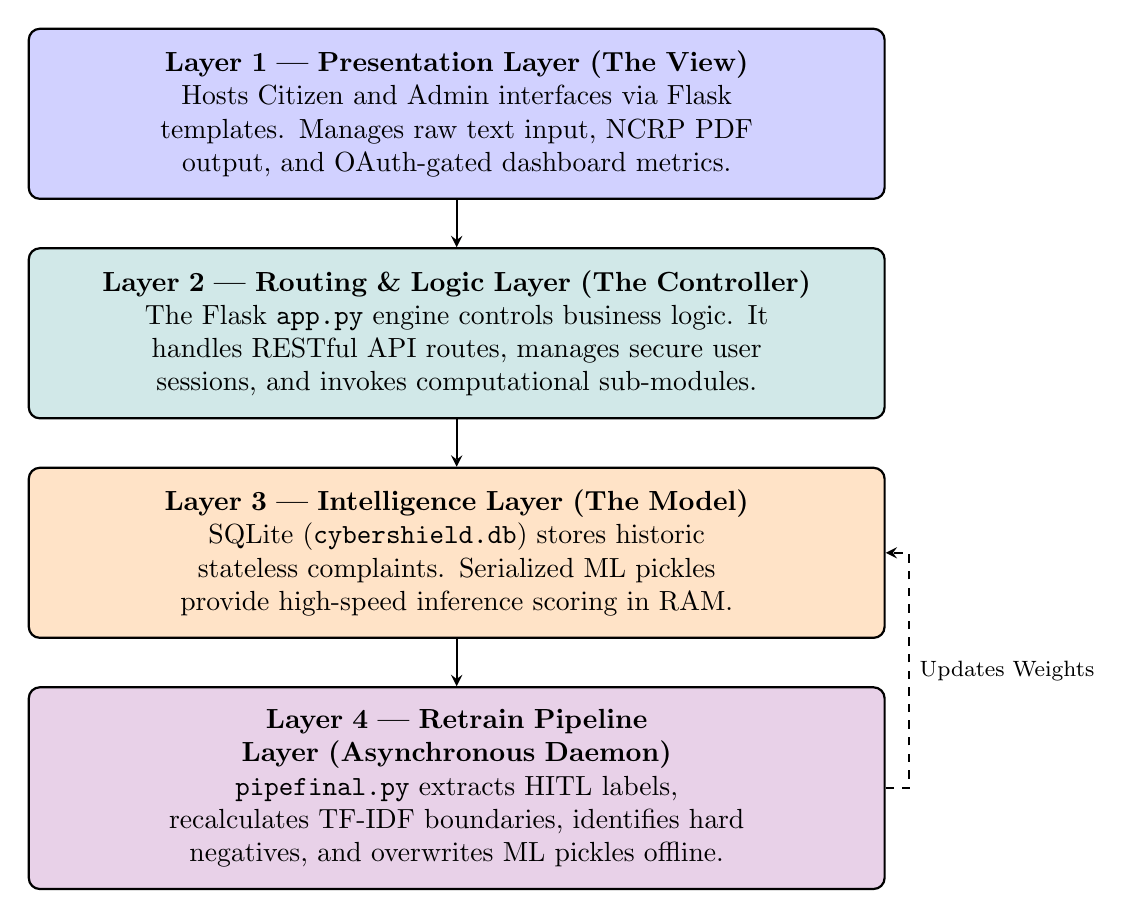
\begin{tikzpicture}[
        node distance=0.6cm,
        layer/.style={
            rectangle, draw=black, thick, text=black,
            text width=0.85\textwidth, align=center, rounded corners,
            minimum height=1.5cm, inner sep=8pt
        },
        arrow/.style={thick, ->, >=stealth, draw=black}
    ]
    
    \node[layer, fill=blue!18] (view) {\textbf{Layer 1 --- Presentation Layer (The View)}\\Hosts Citizen and Admin interfaces via Flask templates. Manages raw text input, NCRP PDF output, and OAuth-gated dashboard metrics.};
    
    \node[layer, fill=teal!18, below=of view] (controller) {\textbf{Layer 2 --- Routing \& Logic Layer (The Controller)}\\The Flask \texttt{app.py} engine controls business logic. It handles RESTful API routes, manages secure user sessions, and invokes computational sub-modules.};
    
    \node[layer, fill=orange!22, below=of controller] (model) {\textbf{Layer 3 --- Intelligence Layer (The Model)}\\SQLite (\texttt{cybershield.db}) stores historic stateless complaints. Serialized ML pickles provide high-speed inference scoring in RAM.};
    
    \node[layer, fill=violet!18, below=of model] (retrain) {\textbf{Layer 4 --- Retrain Pipeline Layer (Asynchronous Daemon)}\\\texttt{pipefinal.py} extracts HITL labels, recalculates TF-IDF boundaries, identifies hard negatives, and overwrites ML pickles offline.};
    
    \draw[arrow] (view) -- (controller);
    \draw[arrow] (controller) -- (model);
    \draw[arrow] (model) -- (retrain);
    
    \draw[arrow, dashed] (retrain.east) -- ++(0.3,0) |- node[right, pos=0.25, font=\footnotesize] {Updates Weights} (model.east);
    
    \end{tikzpicture}%
    }
    \caption{CyberShield Modular System Architecture --- restructured into a four-layer processing pipeline. Adjacent layers communicate sequentially, while the asynchronous Retrain Daemon operates independently to push updated mathematical weights back into the Intelligence Layer.}
    \label{fig:sys_arch}
\end{figure}

\section{Use Case Analysis}
To map the functional requirements into actionable system workflows, a comprehensive Use Case analysis was conducted. Figure \ref{fig:use_case} illustrates the interaction between the primary actors (Citizen and Administrator), the secondary authentication actor (Google OAuth Server), and the encapsulated processes within the CyberShield system boundary.

\begin{figure}[H]
    \centering
    \resizebox{0.95\textwidth}{!}{
        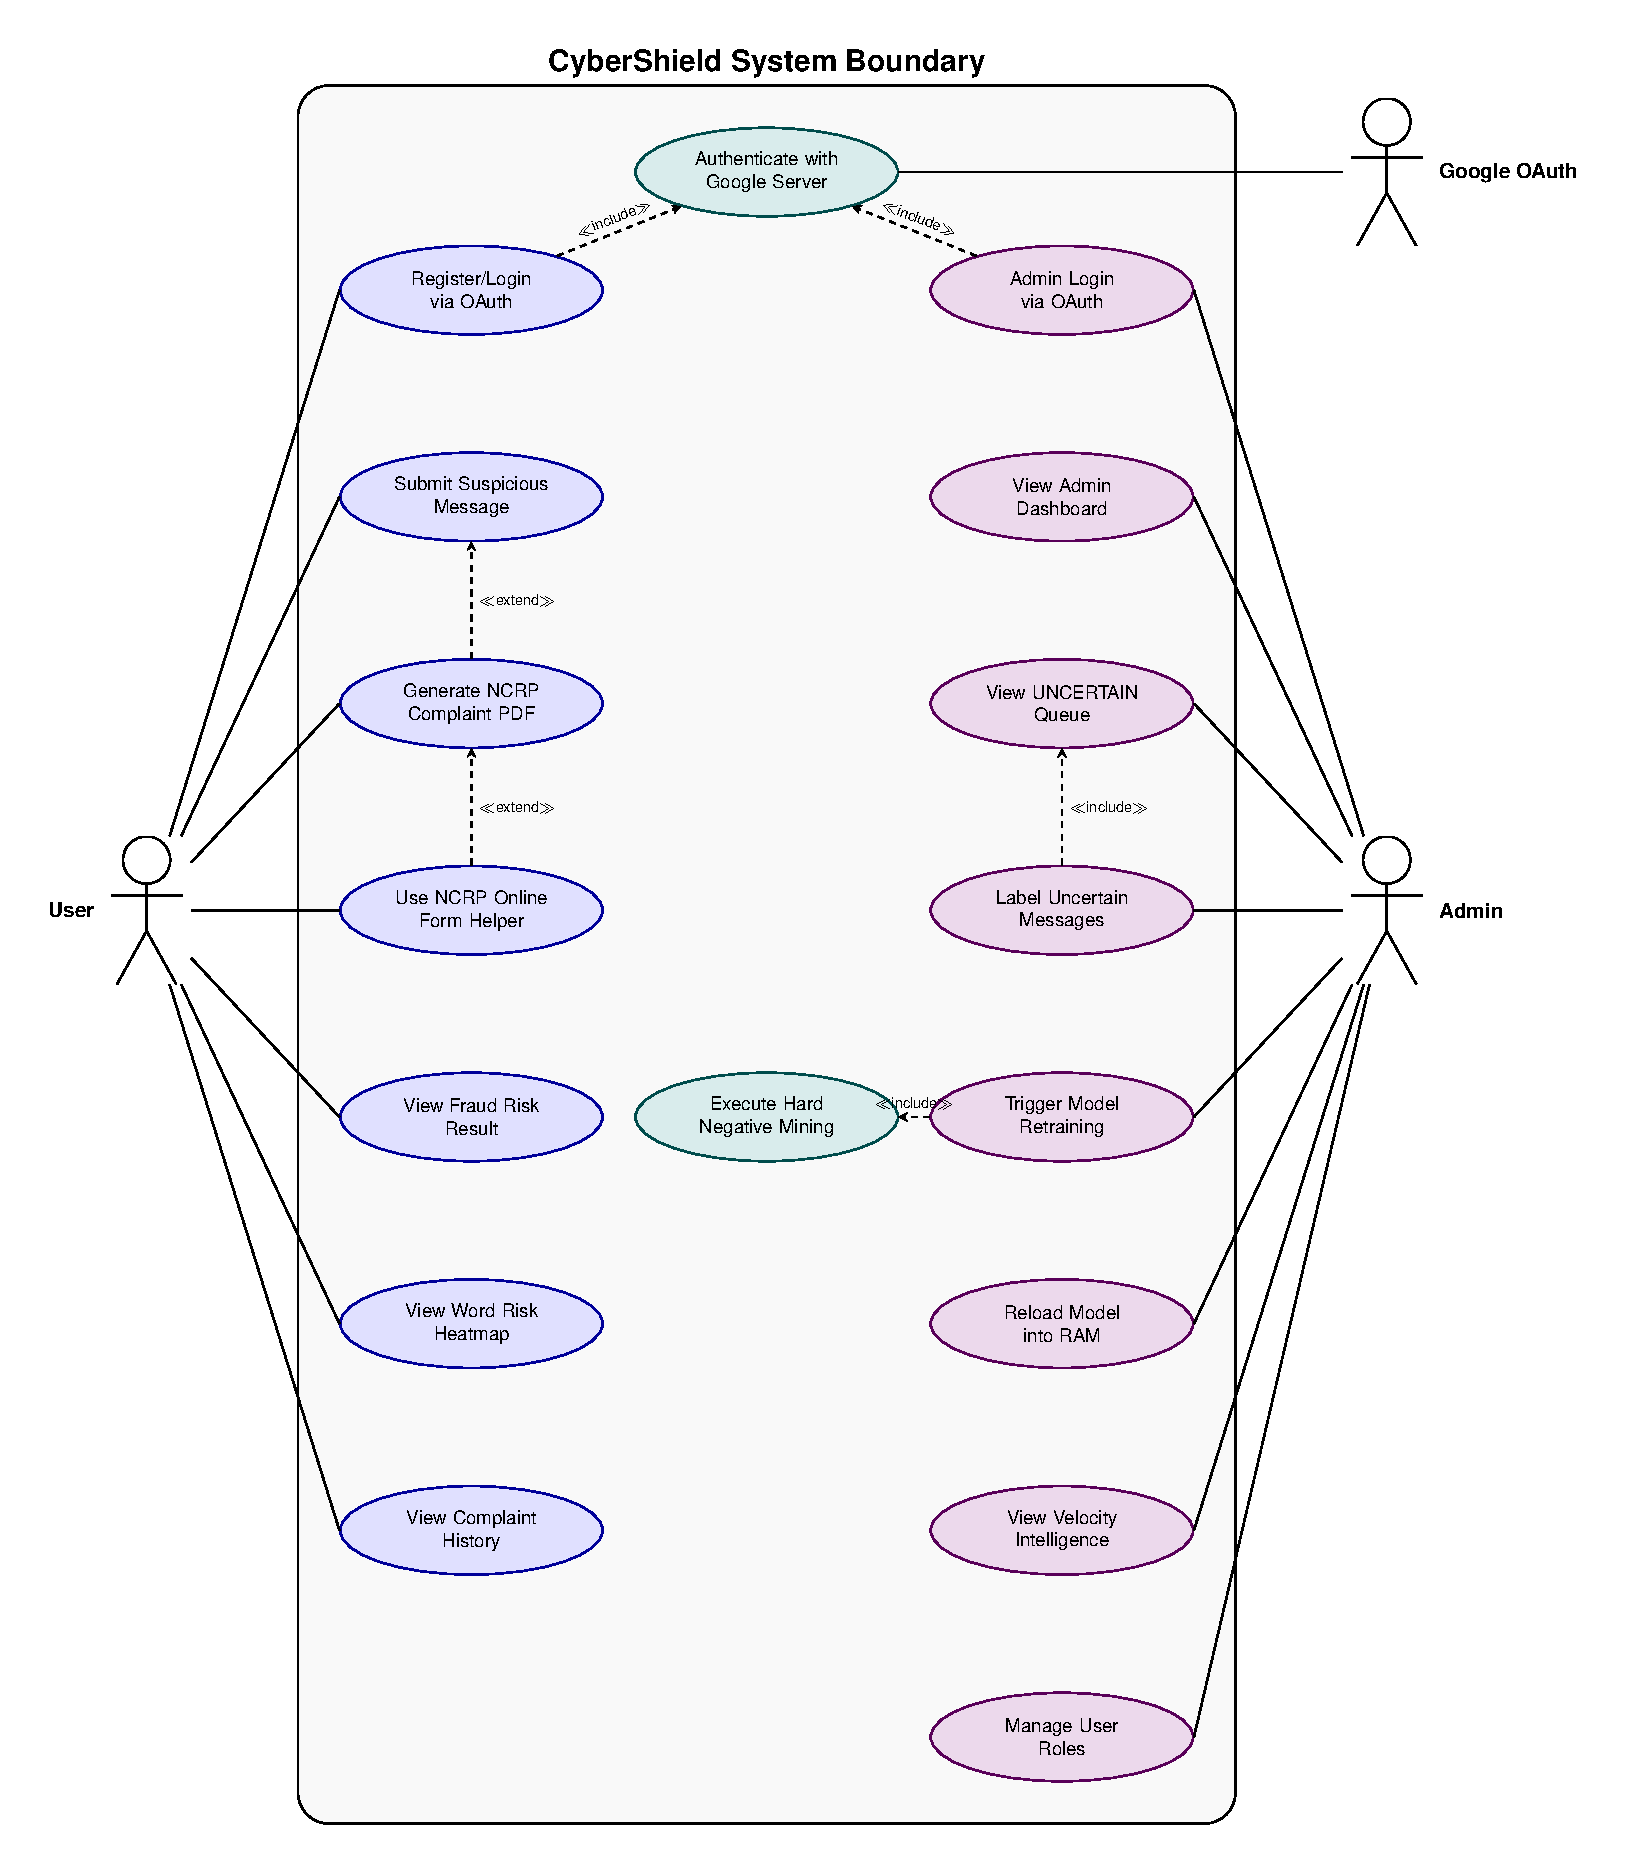
\includegraphics[width=0.85\textwidth]{figures/use_case_diagram.pdf}
    }
    \caption{Formal UML Use Case Diagram for CyberShield --- demonstrating the functional partition between public Citizen workflows and privileged Administrator controls, unified by a central Google OAuth authentication layer.}
    \label{fig:use_case}
\end{figure}

\section{Data Flow Diagrams}
A Data Flow Diagram (DFD) is a structured graphical tool that models the flow of information through a system, its transformations, storage, and interactions with external entities. Two levels are presented here.

\subsection{Level 0 DFD --- Context Diagram}
The Level 0 DFD, also known as the Context Diagram, represents the entire CyberShield system as a single process (Process 0) and defines its boundaries by identifying all external entities that interact with it, along with the high-level data flows between them.

\begin{figure}[H]
    \centering
    \resizebox{\textwidth}{!}{%
        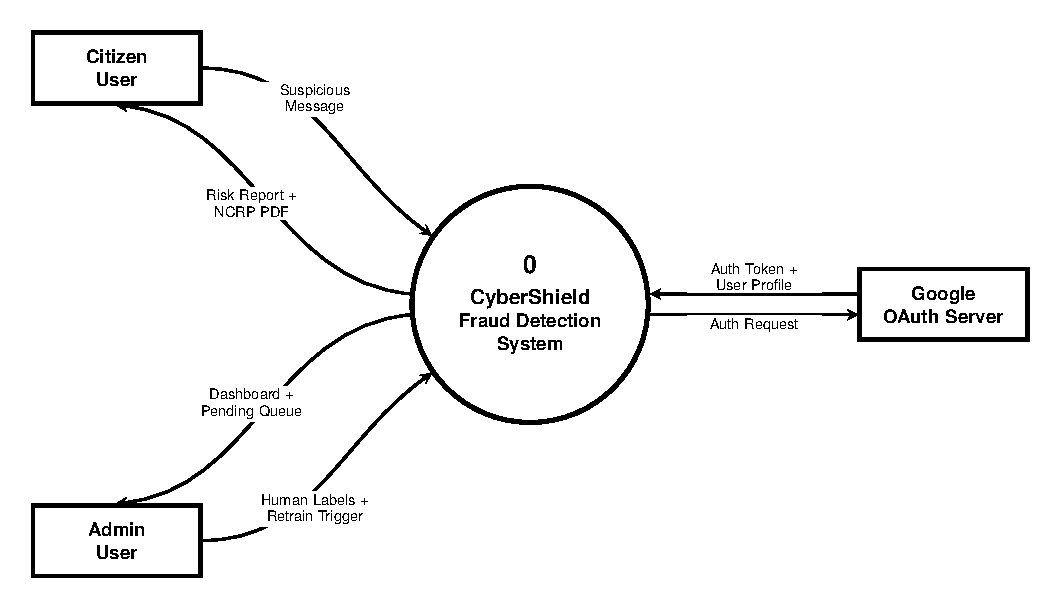
\includegraphics[width=0.85\textwidth]{figures/dfd_level0.pdf}
    }
    \caption{Level 0 DFD (Context Diagram) --- CyberShield system boundary with three external entities: Citizen User, Admin User, and Google OAuth Server, showing high-level input/output data flows.}
    \label{fig:dfd_level0}
\end{figure}

\subsection{Level 1 DFD --- Process Decomposition}
The Level 1 DFD decomposes Process 0 into five distinct functional sub-processes, exposes the four internal data stores, and traces every significant data flow between them and the external entities.

\begin{itemize}
    \item \textbf{P1 --- Authenticate User:} Mediates Google OAuth handshake for both citizen and admin sessions.
    \item \textbf{P2 --- Analyse Message:} Reads ML Models (D4), logs velocity indicators (D2), stores the complaint (D1), and queues uncertain results to D3.
    \item \textbf{P3 --- Generate Report:} Reads D1 to produce the risk heatmap and NCRP PDF returned to the citizen.
    \item \textbf{P4 --- Human Review:} Admin reads D3 (Pending Review DB) and writes human labels back.
    \item \textbf{P5 --- Retrain Model:} Triggered by admin; reads labeled data from D1 and D3, then updates D4 (ML model files).
\end{itemize}

\begin{figure}[H]
    \centering
    \resizebox{\textwidth}{!}{%
        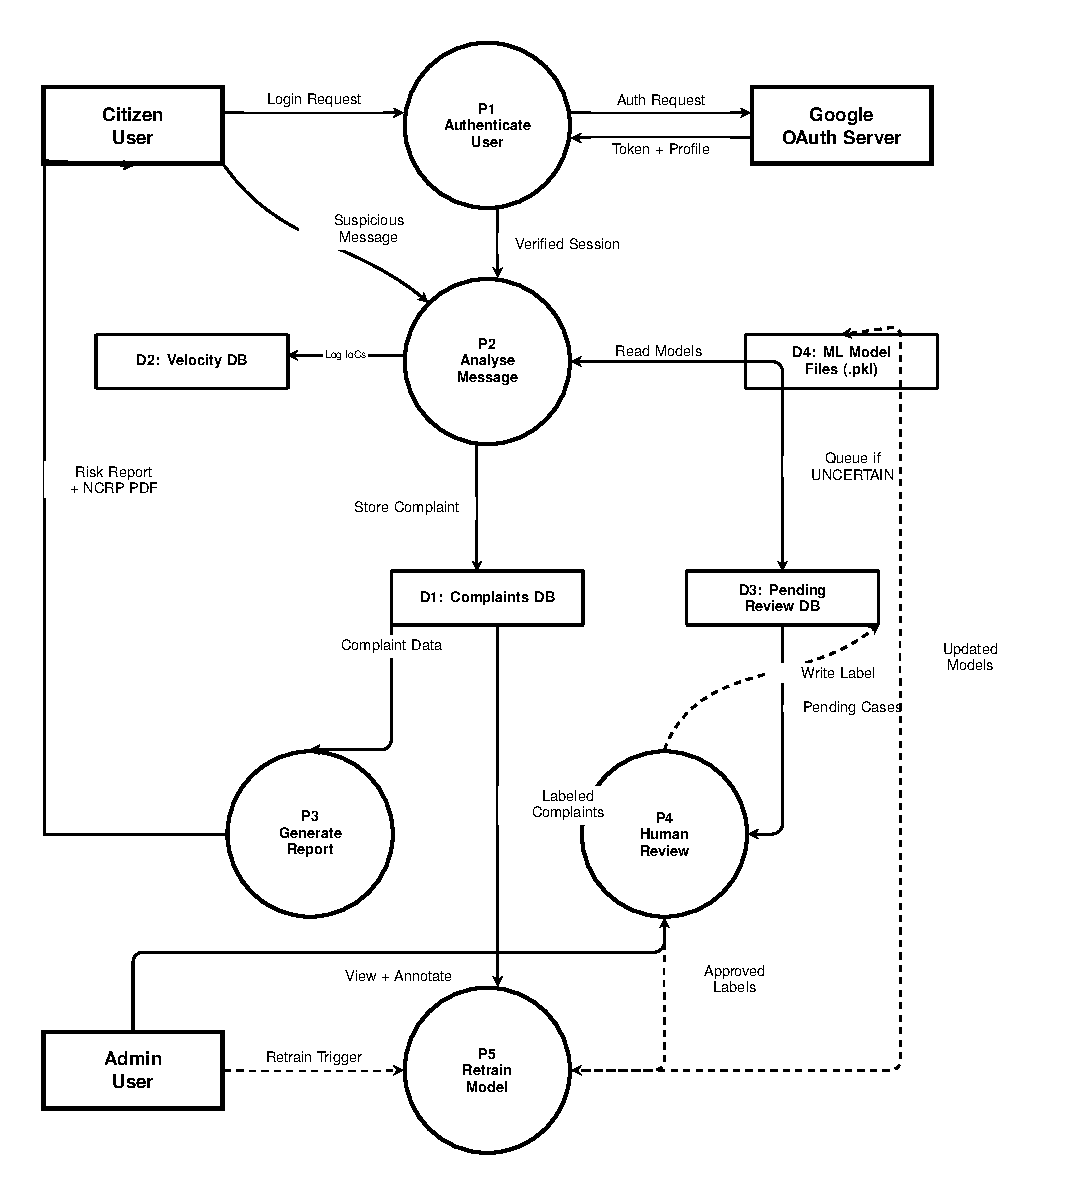
\includegraphics[width=0.85\textwidth]{figures/dfd_level1.pdf}
    }
    \caption{Level 1 DFD --- Decomposition of the CyberShield system into five processes (P1--P5) and four data stores (D1: Complaints, D2: Velocity, D3: Pending Review, D4: ML Models), with all inter-process and entity-to-process data flows.}
    \label{fig:dfd_level1}
\end{figure}

\section{Machine Learning Pipeline Design}
The core intelligence of CyberShield is designed around a three-stage mathematical pipeline: Preprocessing, Vectorization, and Ensemble Modeling.

\subsection{Preprocessing and Feature Extraction}
Raw text input is highly volatile. Before vectors can be mapped, the text undergoes:
\begin{enumerate}
    \item \textbf{Artifact Extraction:} The \texttt{preprocess()} function uses regular expressions to parse out and replace artifacts with semantic placeholder tokens rather than stripping them entirely. Specifically: URLs $\rightarrow$ \texttt{SUSPICIOUS\_URL}, Indian phone numbers (starting with 7/8/9) $\rightarrow$ \texttt{PHONE\_NUMBER}, rupee amounts $\rightarrow$ \texttt{MONEY\_AMOUNT}, USD amounts $\rightarrow$ \texttt{MONEY\_AMOUNT\_USD}, and 4--6 digit OTP patterns $\rightarrow$ \texttt{OTP\_NUMBER}. These tokens are retained as high-value fraud-signal features for the vectorizer.
    \item \textbf{Standardization:} Text is converted to lowercase, newline characters are stripped, and non-alphanumeric punctuation is removed to normalize the feature space.
\end{enumerate}

\begin{figure}[H]
    \centering
    \resizebox{\textwidth}{!}{
    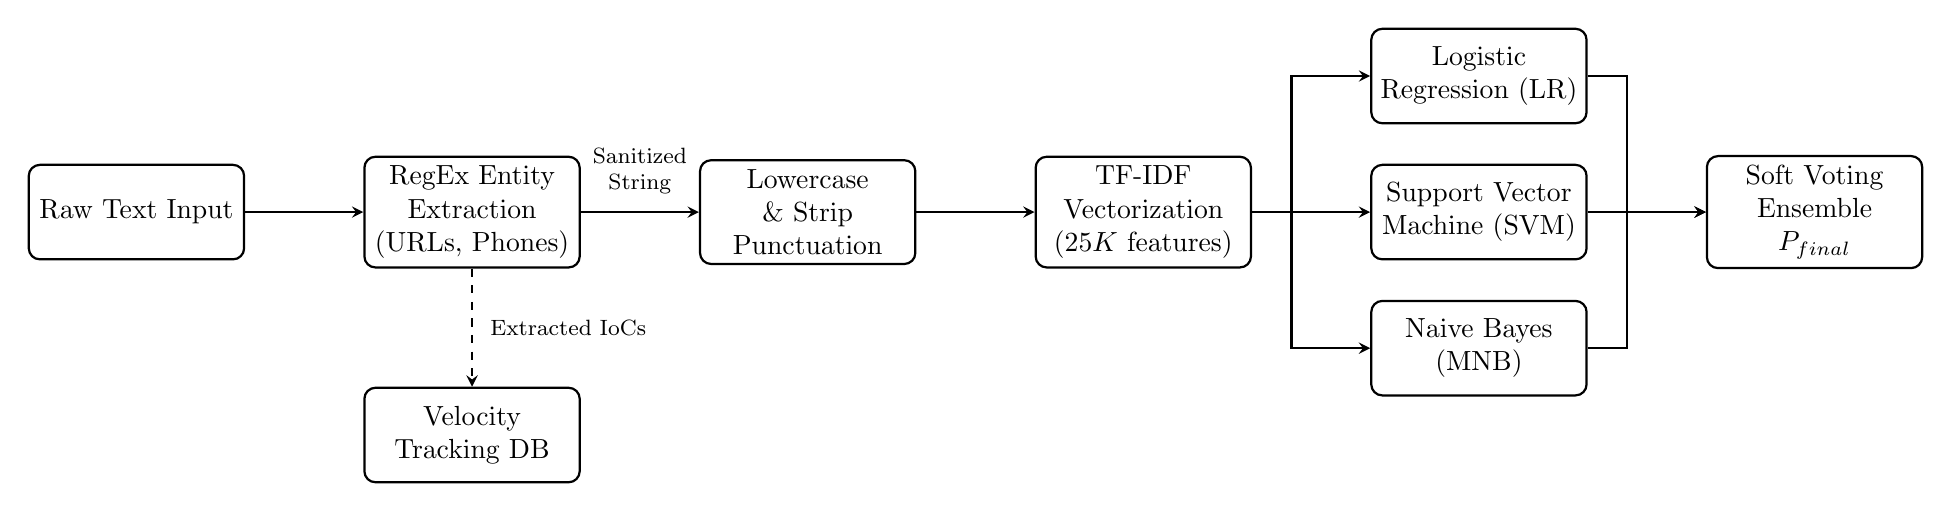
\begin{tikzpicture}[
        node distance=1.5cm and 1.5cm,
        block/.style={rectangle, draw=black, thick, fill=white, text=black, text width=2.5cm, align=center, minimum height=1.2cm, rounded corners},
        arrow/.style={thick, ->, >=stealth, draw=black}
    ]
    \node[block] (raw) {Raw Text Input};
    \node[block, right=of raw] (regex) {RegEx Entity Extraction (URLs, Phones)};
    \node[block, below=of regex] (velocity) {Velocity Tracking DB};
    \node[block, right=of regex] (lower) {Lowercase \& Strip Punctuation};
    \node[block, right=of lower] (tfidf) {TF-IDF Vectorization ($25K$ features)};
    
    \node[block, right=of tfidf] (svm) {Support Vector Machine (SVM)};
    \node[block, above=0.5cm of svm] (lr) {Logistic Regression (LR)};
    \node[block, below=0.5cm of svm] (nb) {Naive Bayes (MNB)};
    
    \node[block, right=of svm] (predict) {Soft Voting Ensemble $P_{final}$};
    
    \draw[arrow] (raw) -- (regex);
    \draw[arrow] (regex) -- node[above=0.1cm, font=\footnotesize, align=center] {Sanitized\\String} (lower);
    \draw[arrow, dashed] (regex) -- node[right=0.1cm, font=\footnotesize] {Extracted IoCs} (velocity);
    \draw[arrow] (lower) -- (tfidf);
    
    \draw[arrow] (tfidf.east) -- ++(0.5,0) |- (lr.west);
    \draw[arrow] (tfidf.east) -- (svm.west);
    \draw[arrow] (tfidf.east) -- ++(0.5,0) |- (nb.west);
    
    \draw[arrow] (lr.east) -- ++(0.5,0) |- (predict.west);
    \draw[arrow] (svm.east) -- (predict.west);
    \draw[arrow] (nb.east) -- ++(0.5,0) |- (predict.west);
    \end{tikzpicture}
    }
    \caption{Level-1 Data Flow Diagram (DFD) of the ML Inference Loop --- illustrating the transformation of raw user input through artifact extraction, text sanitization, TF-IDF vectorization, and soft-voting ensemble scoring to produce the final probabilistic risk output $P_{final}$.}
    \label{fig:dfd}
\end{figure}

\subsection{TF-IDF Vectorization}
Term Frequency-Inverse Document Frequency (TF-IDF) represents words numerically \cite{salton1988term}. 
\begin{equation}
    \text{TF}(t, d) = \log(1 + f_{t,d})
\end{equation}
\begin{equation}
    \text{IDF}(t, D) = \log\left(\frac{N}{|\{d \in D : t \in d\}|}\right)
\end{equation}

\textbf{Notation Legend:}
\begin{itemize}
    \item $t$: A specific term (word or n-gram) in the vocabulary.
    \item $d$: A single document (message).
    \item $D$: The entire corpus of training documents.
    \item $N$: The total number of documents in the corpus.
    \item $f_{t,d}$: The raw frequency count of term $t$ in document $d$.
\end{itemize}

The implementation utilizes a Scikit-learn \texttt{FeatureUnion} \cite{pedregosa2011scikit} to combine two distinct vectorization strategies into a single $25,000$-feature space. The first component is a word n-gram vectorizer (\texttt{ngram\_range=(1,2)}, \texttt{max\_features=20000}, \texttt{sublinear\_tf=True}) with custom stopwords to capture semantic meaning. The second component is a character n-gram vectorizer (\texttt{analyzer='char\_wb'}, \texttt{ngram\_range=(3,5)}, \texttt{max\_features=5000}). This combined approach limits the vocabulary space due to RAM constraints (approximately 1GB) while the character n-grams explicitly provide robustness against adversarial obfuscation attacks (e.g., intentional misspellings).

\subsection{Soft-Voting Ensemble Logic}
An ensemble model prevents the weaknesses of any single algorithm from derailing the prediction \cite{dietterich2000ensemble}. The design utilizes:
\begin{itemize}
    \item \textbf{Logistic Regression (LR):} Provides highly calibrated probabilities \cite{cox1958regression}. Weight = 0.2
    \item \textbf{Support Vector Machine (SVM):} Deployed with a linear kernel, exceptionally proficient at drawing hyperplanes through high-dimensional text matrices \cite{cortes1995support}. Weight = 0.5
    \item \textbf{Multinomial Naive Bayes (MNB):} Calculates conditional probabilities based on Bayes' theorem, serving as a rapid baseline sanity check \cite{mccallum1998comparison}. Weight = 0.3
\end{itemize}

These weights are automatically tuned via a grid search over all valid weight triplets on the validation set during each retraining cycle, selecting the combination that maximizes macro-F1. The weights shown below represent the empirically optimal values from the current training run, not a manually fixed assignment. The final predictive probability is computed as shown in Equation \ref{eq:ensemble}:
\begin{equation}
\label{eq:ensemble}
    P_{final}(Fraud) = (0.2 \times P_{LR}) + (0.5 \times P_{SVM}) + (0.3 \times P_{NB})
\end{equation}
where $P_{final}(Fraud)$ is the ensembled probability score, and $P_{LR}$, $P_{SVM}$, and $P_{NB}$ are the individual fraud probabilities predicted by the Logistic Regression, Support Vector Machine, and Naive Bayes classifiers, respectively.

\section{Database Design}
CyberShield operates a lightweight SQLite database designed for rapid reads and simple structured queuing.
The schema logic comprises two primary operational architectures:

\subsection{User Identity and Authorization Schema}
The \texttt{users} table serves as the primary authentication and role-management ledger. Integrated with Google OAuth 2.0, this table tracks user identity and access privileges without storing sensitive passwords. Key fields include the user's primary email address, display name, and an administrative role flag. This table ensures that access to the Human-in-the-Loop (HITL) adjudication dashboard and retraining pipelines is strictly restricted to authorized administrators, preventing malicious actors from poisoning the active model.

\subsection{Citizen Submission and Routing Schema}
The v4 SQLAlchemy schema normalizes the database into four distinct tables: \texttt{users}, \texttt{complaints}, \texttt{velocity\_db}, and \texttt{pending\_review}. The \texttt{complaints} table acts as the historic lookup ledger for generated PDFs. The Human-in-the-Loop adjudication fields (\texttt{admin\_label} and \texttt{labeled\_by}) now reside exclusively in the \texttt{pending\_review} table. Figure \ref{fig:er_diagram} provides a visual representation of this normalized schema and its relationships. Table \ref{tab:complaints_schema} outlines the expanded fields of the \texttt{complaints} table.

\begin{table}[H]
    \centering
    \resizebox{\textwidth}{!}{
    \begin{tabular}{|l|l|l|l|}
    \hline
    \textbf{Column Name} & \textbf{Data Type} & \textbf{Constraint} & \textbf{Description} \\ \hline
    id & INTEGER & Primary Key, Auto-increment & Internal index tracker. \\ \hline
    user\_id & INTEGER & Foreign Key & Links complaint to a registered user. \\ \hline
    complaint\_id & VARCHAR(16) & Unique, Not Null & Hexadecimal UUID given to user. \\ \hline
    message & TEXT & Not Null & Raw string input payload. \\ \hline
    fraud\_probability & REAL & Range [0.0, 1.0] & Mathematical probability score. \\ \hline
    risk\_level & VARCHAR(12) & ENUM Constraint & FRAUD, SUSPICIOUS, UNCERTAIN, or LEGIT. \\ \hline
    fraud\_category & VARCHAR(50) & Nullable & Matched NCRP fraud category. \\ \hline
    ncrp\_code & VARCHAR(20) & Nullable & Generated NCRP Complaint Category Code. \\ \hline
    phones\_found & TEXT & Nullable & JSON array of extracted phone numbers. \\ \hline
    urls\_found & TEXT & Nullable & JSON array of extracted URLs. \\ \hline
    amounts\_found & TEXT & Nullable & JSON array of extracted monetary amounts. \\ \hline
    otps\_found & TEXT & Nullable & JSON array of extracted OTPs. \\ \hline
    keywords & TEXT & Nullable & JSON array of high-risk keywords. \\ \hline
    velocity\_alerts & TEXT & Nullable & JSON array of velocity tracking alerts. \\ \hline
    complainant\_name & VARCHAR(100) & Nullable & Name of the victim filing the report. \\ \hline
    complainant\_contact & VARCHAR(100) & Nullable & Contact information of the victim. \\ \hline
    sender & VARCHAR(100) & Nullable & Claimed sender of the malicious message. \\ \hline
    pdf\_path & VARCHAR(255) & Nullable & File path to the generated NCRP PDF. \\ \hline
    \end{tabular}
    }
    \caption{Entity-Relationship schema of the \texttt{complaints} table, illustrating the structural linkage between citizen submissions, extracted threat vectors, and assigned probabilistic risk scores.}
    \label{tab:complaints_schema}
\end{table}

\subsection{Velocity Tracking and Threat Intelligence Schema}
Velocity tracking in v4 is handled natively by the \texttt{velocity\_db} SQLAlchemy table rather than a flat JSON file, leveraging the ORM for concurrency management. The schema includes the following columns: \texttt{id} (Primary Key), \texttt{indicator\_type} (e.g., phone, url), \texttt{indicator\_value} (the artifact string), \texttt{count} (total hits), \texttt{complaint\_ids} (a JSON array of linked complaint IDs for traceability), \texttt{first\_seen} (timestamp), and \texttt{last\_seen} (timestamp). To ensure data integrity, a unique constraint is applied to the composite tuple \texttt{(indicator\_type, indicator\_value)}.

The velocity intelligence system assigns three formally defined threat tiers based on the cumulative occurrence count of each artifact across independent submissions:
\begin{itemize}
    \item \textbf{MED (count $= 1$):} An artifact encountered for the first time. MED represents a monitoring flag rather than an action trigger---the artifact is logged and tracked but does not yet constitute evidence of coordinated malicious activity.
    \item \textbf{HIGH (count $\geq 2$):} An artifact appearing across two or more independent victim submissions. A single malicious artifact seen across two independent reports indicates coordinated fraud activity rather than coincidence.
    \item \textbf{CRITICAL (count $\geq 4$):} A pragmatic operational threshold above which the artifact should be treated as an active campaign indicator warranting immediate administrative intervention.
\end{itemize}
These thresholds are heuristic and are recommended for empirical calibration against live deployment data in future iterations.

\subsection{Human-in-the-Loop Adjudication Queue Schema}
The \texttt{pending\_review} table is the operational core of the Human-in-the-Loop calibration system. It acts as an isolation queue for all messages classified as UNCERTAIN ($0.30 \leq P(Fraud) < 0.70$). Rather than polluting the historical \texttt{complaints} ledger with unverified machine annotations, ambiguous cases are safely parked here. The schema includes fields for the raw message, the initial model probabilities, and critical adjudication fields: \texttt{admin\_label} (the final human verdict) and \texttt{labeled\_by} (tracking which administrator made the decision for audit purposes). Once adjudicated, these records are harvested by the \texttt{pipefinal.py} script for Hard Negative Mining.

\begin{figure}[H]
    \centering
    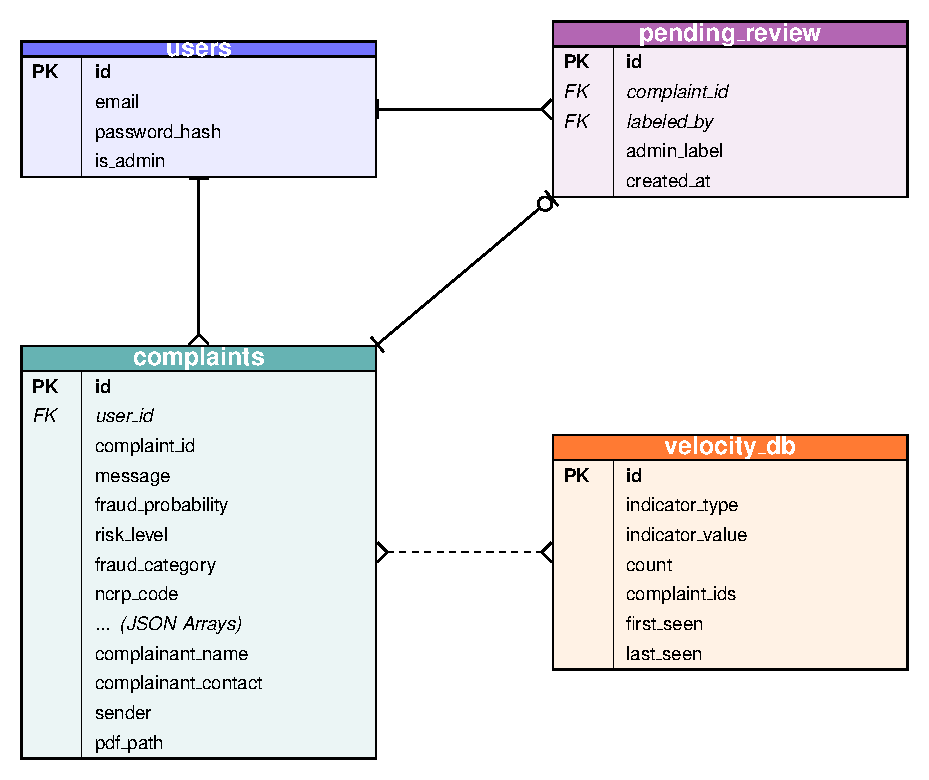
\includegraphics[width=0.85\textwidth]{figures/er_diagram.pdf}
    \caption{Entity-Relationship diagram of the v4 CyberShield database schema, outlining the linkages between users, complaints, velocity tracking, and manual annotations.}
    \label{fig:er_diagram}
\end{figure}

\section{Human-in-the-Loop (HITL) Design Workflow}
Traditional systems are fully autonomous. CyberShield is designed as a semi-autonomous calibration loop that acknowledges uncertainty \cite{holzinger2016interactive}. The workflow proceeds as follows:
\begin{enumerate}
    \item \textbf{Inference:} User submits a message. $P_{final}$ calculates to $0.42$.
    \item \textbf{Routing:} The threshold logic catches $0.42$ in the $0.30 - 0.70$ boundary. Risk is set to UNCERTAIN.
    \item \textbf{Queuing:} The record is saved in the \texttt{complaints} table with \texttt{admin\_label = NULL}.
    \item \textbf{Adjudication:} An Admin logs into \texttt{/admin}. The dashboard queries all records where \texttt{admin\_label} is NULL. The admin reads the context and officially tags it as `fraud`.
    \item \textbf{Mining:} When the admin triggers \texttt{Retrain Model}, the \texttt{pipefinal.py} script awakens. It queries the DB for all non-NULL \texttt{admin\_label} entries.
    \item \textbf{Training Integration:} These newly labeled samples are strictly injected into the Training array. The model undergoes vectorization and applies Hard Negative Mining algorithms, significantly adjusting the decision boundary to guarantee that similar linguistic patterns will permanently register above $0.90$ probability in the future.
    \item \textbf{Model Activation:} Upon successful completion of \texttt{pipefinal.py}, the new \texttt{final\_models.pkl} and \texttt{final\_vectorizer.pkl} are written to disk. The admin clicks the Reload Model button, which triggers the \texttt{/admin/reload-model} route, hot-loading the new pickle files into RAM without requiring a server restart.
\end{enumerate}

\begin{figure}[H]
    \centering
    \resizebox{\textwidth}{!}{
    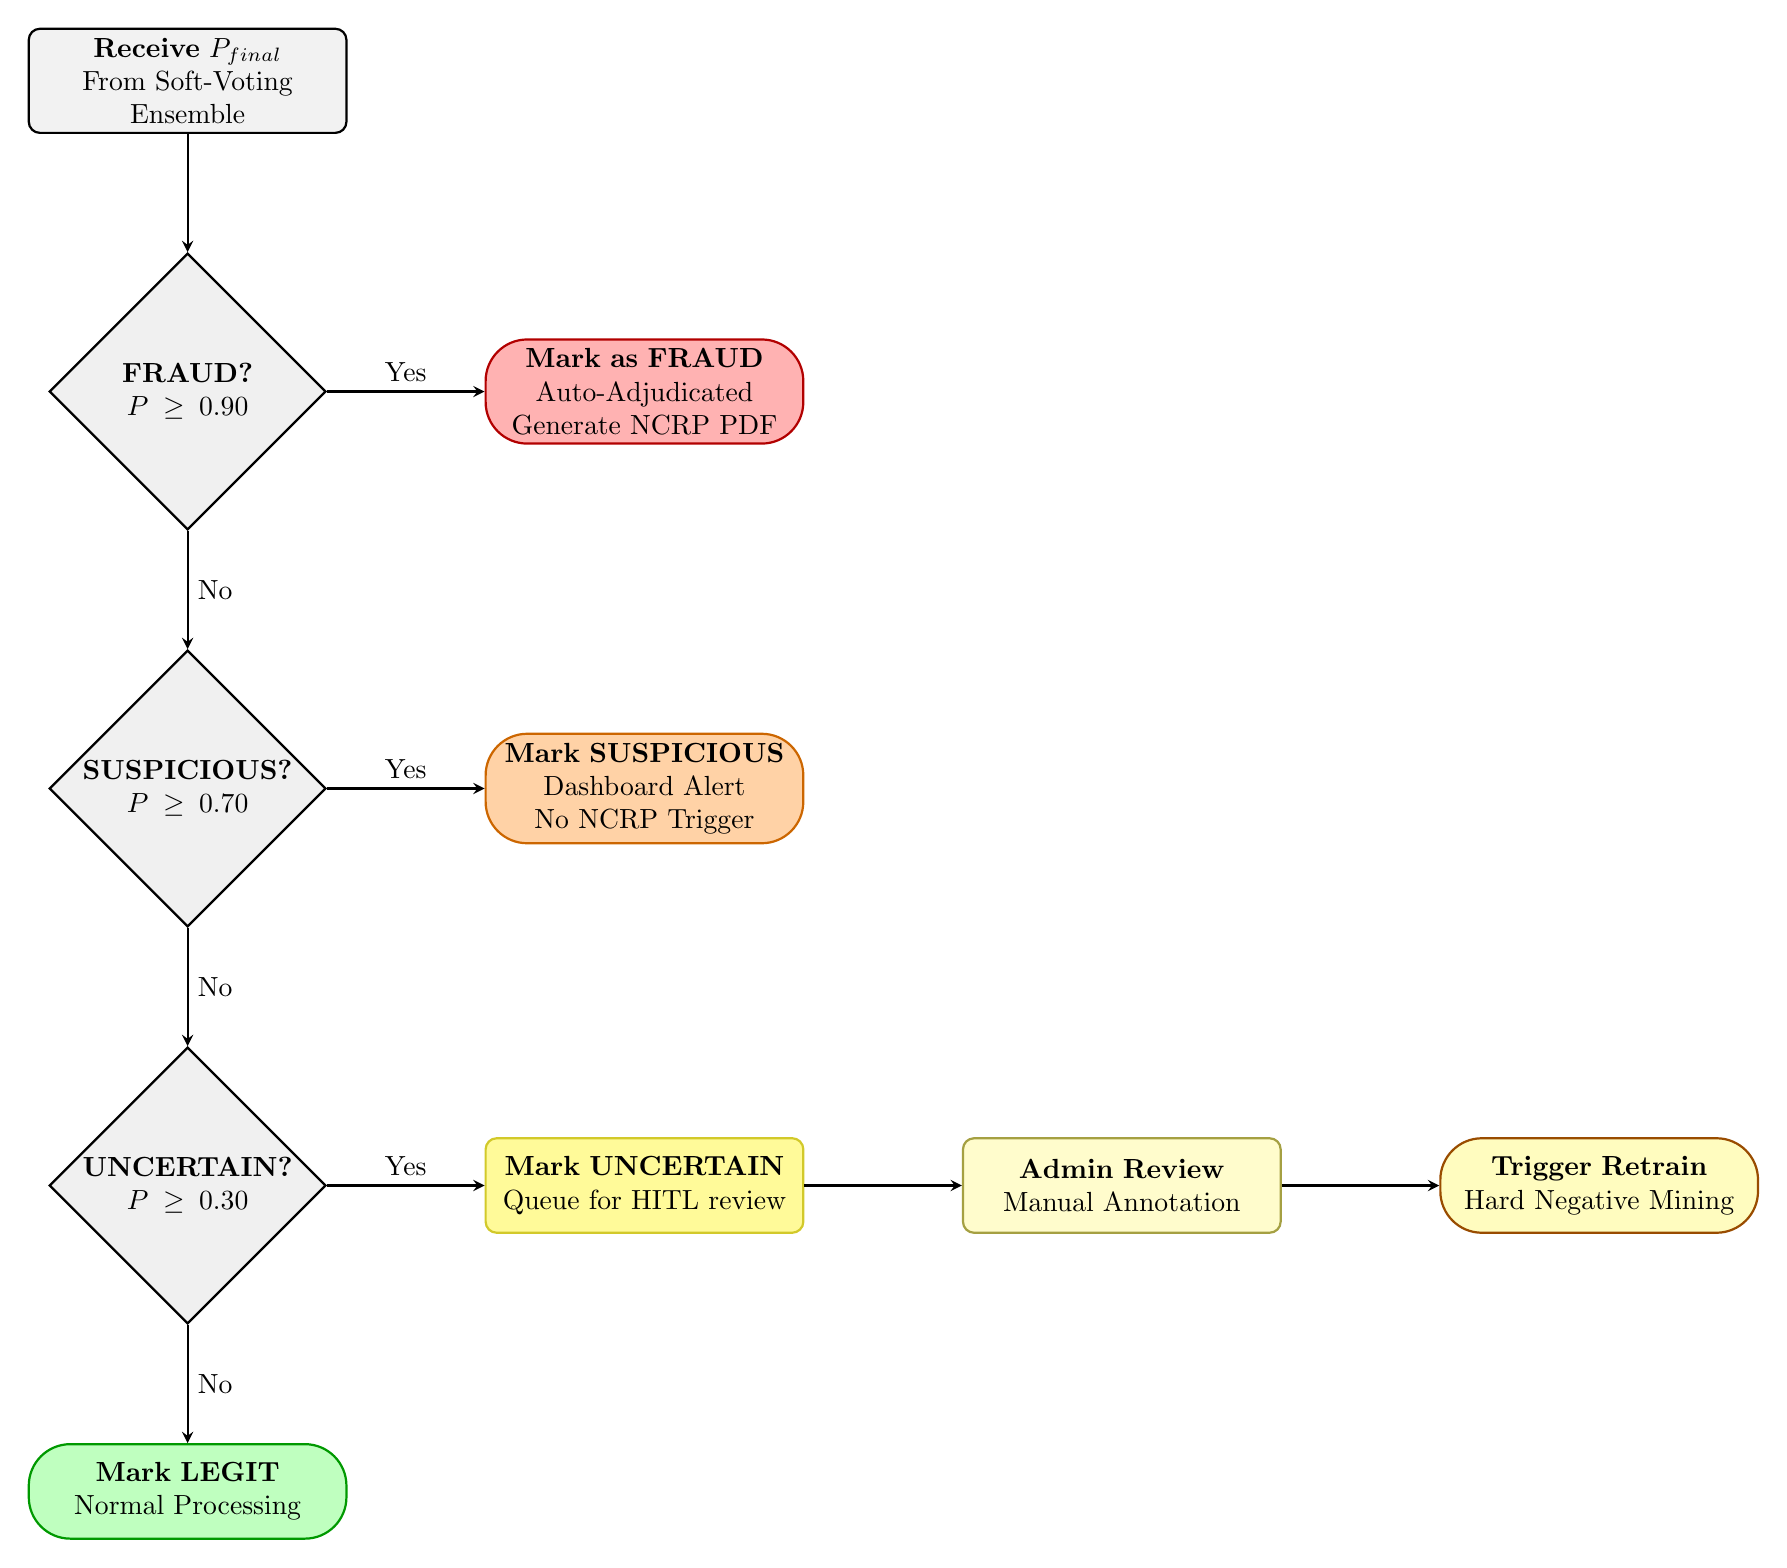
\begin{tikzpicture}[
        node distance=1.5cm and 2cm,
        decision/.style={diamond, draw, thick, text width=2.8cm, align=center, inner sep=0pt, fill=gray!12},
        block/.style={rectangle, draw, thick, text width=3.8cm, align=center, rounded corners, minimum height=1.2cm, fill=white},
        term/.style={rectangle, draw, thick, text width=3.8cm, align=center, rounded corners=15pt, minimum height=1.2cm},
        arrow/.style={thick, ->, >=stealth}
    ]
    
    \node[block, fill=gray!10] (input) {\textbf{Receive $P_{final}$}\\From Soft-Voting Ensemble};
    \node[decision, below=of input] (d1) {\textbf{FRAUD?}\\$P \geq 0.90$};
    \node[term, right=of d1, fill=red!30, draw=red!70!black] (fraud) {\textbf{Mark as FRAUD}\\Auto-Adjudicated\\Generate NCRP PDF};
    
    \node[decision, below=of d1] (d2) {\textbf{SUSPICIOUS?}\\$P \geq 0.70$};
    \node[term, right=of d2, fill=orange!35, draw=orange!80!black] (susp) {\textbf{Mark SUSPICIOUS}\\Dashboard Alert\\No NCRP Trigger};
    
    \node[decision, below=of d2] (d3) {\textbf{UNCERTAIN?}\\$P \geq 0.30$};
    \node[block, right=of d3, fill=yellow!40, draw=yellow!80!black] (unc) {\textbf{Mark UNCERTAIN}\\Queue for HITL review};
    \node[block, right=of unc, fill=yellow!20, draw=yellow!60!black] (admin) {\textbf{Admin Review}\\Manual Annotation};
    \node[term, right=of admin, fill=yellow!25, draw=orange!60!black] (retrain) {\textbf{Trigger Retrain}\\Hard Negative Mining};
    
    \node[term, below=of d3, fill=green!25, draw=green!60!black] (legit) {\textbf{Mark LEGIT}\\Normal Processing};
    
    \draw[arrow] (input) -- (d1);
    \draw[arrow] (d1) -- node[above] {Yes} (fraud);
    \draw[arrow] (d1) -- node[right] {No} (d2);
    
    \draw[arrow] (d2) -- node[above] {Yes} (susp);
    \draw[arrow] (d2) -- node[right] {No} (d3);
    
    \draw[arrow] (d3) -- node[above] {Yes} (unc);
    \draw[arrow] (d3) -- node[right] {No} (legit);
    
    \draw[arrow] (unc) -- (admin);
    \draw[arrow] (admin) -- (retrain);
    \end{tikzpicture}
    }
    \caption{Human-in-the-Loop Threshold Decision Flowchart --- showing the four-tier probabilistic routing logic. Messages with $P_{final} \geq 0.90$ are auto-adjudicated as FRAUD; those between $0.70\text{--}0.90$ as SUSPICIOUS; those between $0.30\text{--}0.70$ are queued as UNCERTAIN for human review and subsequent Hard Negative Mining retraining; those below $0.30$ are marked LEGIT.}
    \label{fig:hitl}
\end{figure}

\section{Serialized Artifact Design}
The intelligence of CyberShield does not persist within standard relational tables but is serialized into highly compressed binary files utilizing the \texttt{pickle} and \texttt{joblib} modules. The architecture mandates three distinct serialized artifacts:
\begin{itemize}
    \item \texttt{split\_indices.pkl}: Stores frozen integer index arrays for the Train, Validation, and Test splits. This artifact guarantees data continuity and mathematical reproducibility across infinite retraining cycles.
    \item \texttt{final\_vectorizer.pkl}: Stores the fitted \texttt{TfidfVectorizer} object comprising the $25,000$-feature vocabulary, fitted exclusively on the training array subset.
    \item \texttt{final\_models.pkl}: Stores the three fitted classifier objects (LR, SVM, NB) along with their calibration wrappers to ensure accurate probabilistic outputs.
\end{itemize}
These files are aggressively written to the disk subsystem by \texttt{pipefinal.py} post-training. During the boot sequence, the Flask application (\texttt{app.py}) ingests these files entirely into RAM. Therefore, overwriting these files is the explicit mechanism by which the retraining module updates the live inference system without requiring database migrations.

\section{API Route Design}
The system routes interact via standard REST protocols. Table \ref{tab:api_routes} defines the primary endpoints driving the CyberShield web architecture.

\begin{table}[H]
    \centering
    \resizebox{\textwidth}{!}{
    \begin{tabular}{|l|l|l|l|}
    \hline
    \textbf{Route} & \textbf{Method} & \textbf{Auth Required} & \textbf{Purpose} \\ \hline
    \texttt{/} & GET & No & Serves the citizen-facing home interface. \\ \hline
    \texttt{/analyze} & POST & Yes (Google OAuth) & Accepts raw text, returns probabilistic risk and extracted artifacts. \\ \hline
    \texttt{/generate-pdf} & POST & Yes (Google OAuth) & Generates NCRP-compliant PDF; \texttt{complaint\_id} must belong to the requesting user. \\ \hline
    \texttt{/download-complaint/<id>} & GET & Yes (Google OAuth) & Downloads the PDF; validates \texttt{complaint\_id} ownership before serving. \\ \hline
    \texttt{/ncrp-helper/<id>} & GET & No & Serves the helper interface for manual NCRP filing. \\ \hline
    \texttt{/history} & GET & Yes & Displays the complaint history for the logged-in user. \\ \hline
    \texttt{/admin} & GET & OAuth (Whitelisted Email) & Serves the admin dashboard showing pending UNCERTAIN queue. \\ \hline
    \texttt{/admin/label} & POST & OAuth (Whitelisted Email) & Writes human annotation (fraud/legit) to a complaint record. \\ \hline
    \texttt{/admin/retrain} & POST & OAuth (Whitelisted Email) & Triggers asynchronous \texttt{pipefinal.py} subprocess to retrain the model. \\ \hline
    \texttt{/admin/reload-model} & POST & Admin & Hot-loads newly trained models into RAM. \\ \hline
    \texttt{/admin/retrain-status} & GET & Admin & Polls the status of the background retraining task. \\ \hline
    \texttt{/admin/velocity-db} & GET & Admin & Serves the Velocity Intelligence threat dashboard. \\ \hline
    \texttt{/admin/users} & GET & Admin & Serves the user management panel. \\ \hline
    \texttt{/admin/users/<id>/toggle-admin} & POST & Admin & Promotes or demotes a user's admin privileges. \\ \hline
    \end{tabular}
    }
    \caption{Overview of defined API routes, detailing HTTP methods, endpoint URIs, and their respective functional purposes within the CyberShield architecture.}
    \label{tab:api_routes}
\end{table}

\section{Failure Mode and Error Handling Design}
To guarantee a resilient production deployment, the architecture proactively defends against the following failure permutations:
\begin{enumerate}
    \item \textbf{Missing Artifacts:} If \texttt{final\_models.pkl} or \texttt{final\_vectorizer.pkl} are missing on server boot, Flask will purposefully raise a fatal startup exception with a descriptive error message rather than failing silently at inference time.
    \item \textbf{Database Concurrency:} SQLAlchemy's connection pool manages concurrent database access, providing thread-safe read/write operations across simultaneous requests without requiring manual WAL configuration.
    \item \textbf{Retrain Subprocess Crash:} If the \texttt{pipefinal.py} retraining subprocess crashes midway (e.g., due to an Out-of-Memory error), the existing pickle files are left completely untouched. The script is programmed to only overwrite the local artifacts upon a fully successful completion routine, meaning partial failures do not corrupt the live model.
    \item \textbf{Conversational False Positives:} Short benign messages (e.g., ``Hi'', ``Thanks'') can cross the 0.30 UNCERTAIN threshold and pollute the admin queue. A deterministic colloquial override forces $P(\text{Fraud}) = 0.05$ for conversational regex matches when the raw ensemble probability is below 0.50, while intentionally leaving predictions above 0.50 unsuppressed to avoid masking genuinely malicious openers.
\end{enumerate}

\section{End-to-End System Pipeline Flow}
Figure~\ref{fig:pipeline_flow} maps the complete data processing pipeline across ten stages and five functional swimlanes: Citizen, Flask Controller, ML Intelligence Layer, SQLite Database, and Administrator. Stages~9 and~10 illustrate the isolated HITL calibration and Hard Negative Mining feedback loop, enabling the model to adapt over time without server restarts.

\begin{figure}[H]
    \centering
    \resizebox{\textwidth}{!}{
        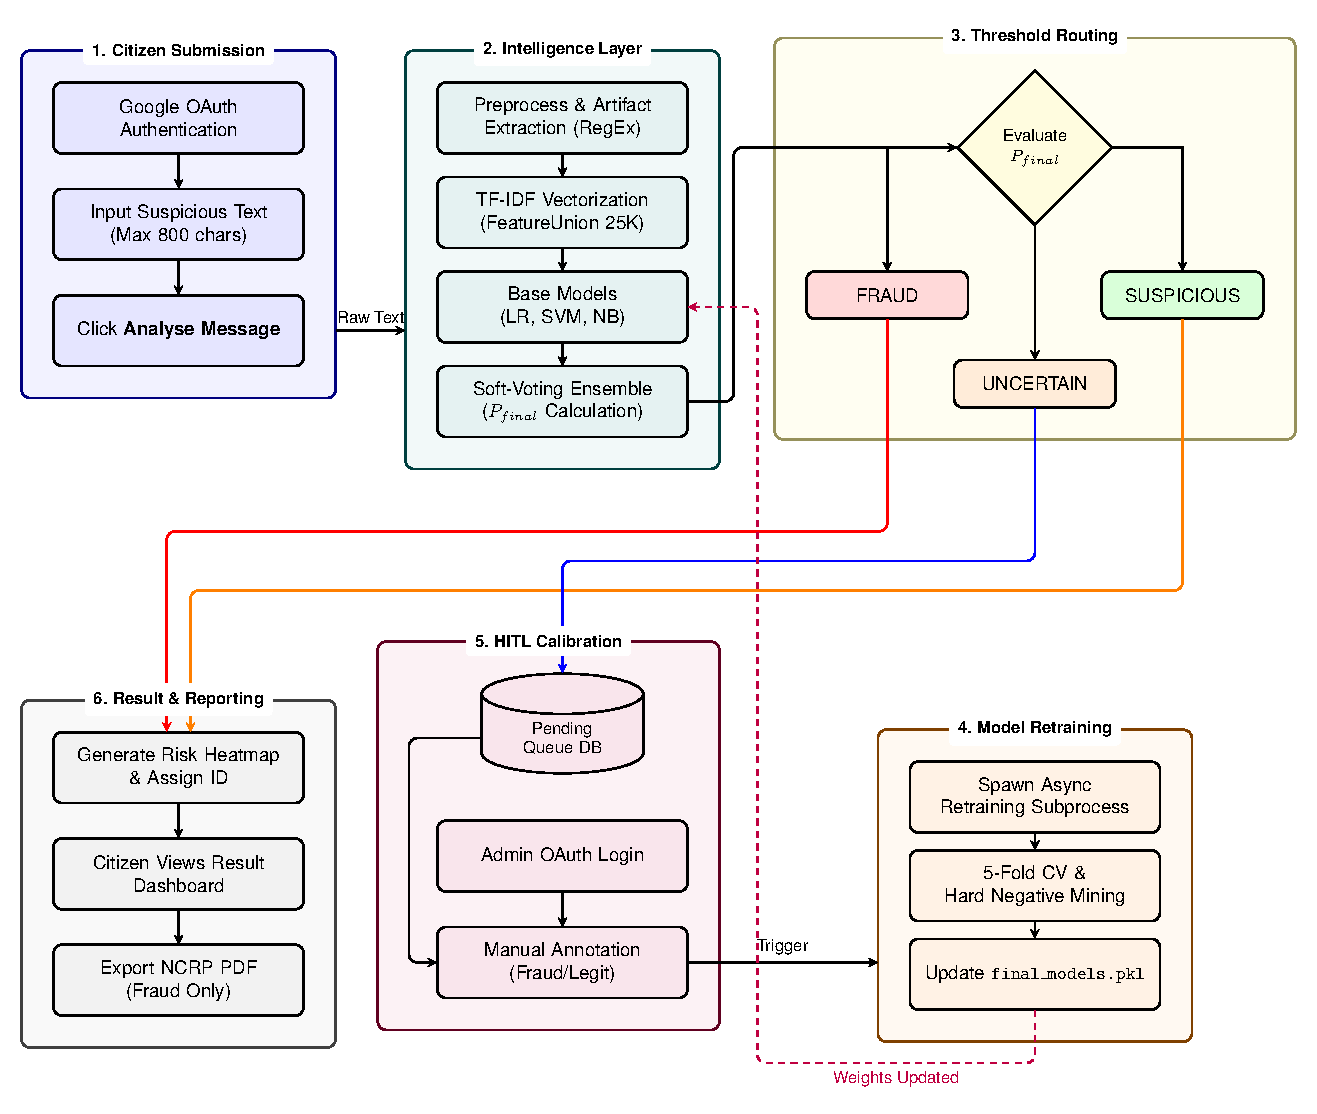
\includegraphics[width=0.85\textwidth]{figures/pipeline_flow.pdf}
    }
    \caption{End-to-End System Pipeline Flow Diagram mapping the 10-stage lifecycle across all architectural layers, including the offline asynchronous retraining loop.}
    \label{fig:pipeline_flow}
\end{figure}

        \chapter{Implementation}
        \section{Introduction}
CyberShield is developed primarily using Python, built on the pandas and scikit-learn stack for machine learning, and the Flask micro-framework for the web server implementation. This chapter describes the implementation modules covering data ingestion, mathematical training, and web serving. The implementation is organized across the following modules: \texttt{pipefinal.py} (offline ML training and HNM pipeline), \texttt{app.py} (Flask web server and inference engine), \texttt{models.py} (SQLAlchemy ORM models for the four database tables defined in Chapter~4), \texttt{config.py} (OAuth whitelist and Flask configuration), and \texttt{templates/} (Jinja2 HTML interfaces for citizen and admin views).

\section{Development Environment and Architectural Decisions}

\paragraph{Why Python and scikit-learn over deep learning frameworks?}
The decision to use Python and scikit-learn was driven by an inference latency budget of 500ms and the explainability requirement for the Word Risk Heatmap via inspectable logistic regression coefficients. Furthermore, this approach eliminates the need for a GPU, significantly lowering the barrier for deployment.

\paragraph{Why a monolithic app.py rather than a microservices architecture?}
A monolithic architecture reduces operational complexity for a single-machine deployment and is easier for supervisors and examiners to read. The serialized pickle artifacts act as the natural service boundary between the offline training loop and the online inference server.

\paragraph{Why pickle/joblib for model serialization rather than ONNX or SavedModel formats?}
Using \texttt{joblib}\footnote{\url{https://joblib.readthedocs.io}} leverages scikit-learn's native format, allowing zero-overhead loading into RAM. This format facilitates hot-reloading via the \texttt{/admin/reload-model} endpoint without requiring a server restart, ensuring seamless model updates.

\paragraph{Why SQLite + SQLAlchemy over raw SQL or a heavier RDBMS?}
SQLite combined with SQLAlchemy provides a zero-configuration, file-based database solution with a connection pool managed by SQLAlchemy for thread safety. This setup is sufficient for the scale of a single-institution deployment without the overhead of maintaining a heavier relational database management system.

\paragraph{Why Flask over Django or FastAPI?}
Flask's micro-framework architecture \cite{grinberg2018flask} minimizes boilerplate while offering built-in Jinja2 templating and seamless integration with \texttt{flask-dance} for OAuth. Furthermore, it avoids Object-Relational Mapping (ORM) lock-in, allowing SQLAlchemy to be added independently as needed.

\paragraph{Why ReportLab for PDF generation rather than WeasyPrint or a browser-based PDF?}
ReportLab\footnote{Official ReportLab documentation: \url{https://www.reportlab.com/docs/reportlab-userguide.pdf}} is a pure Python library with no browser dependencies. Its Canvas API provides pixel-accurate layout capabilities necessary for generating formal government documents, and it operates entirely offline, ensuring privacy and reliability.

\paragraph{Why Google OAuth rather than local username/password auth?}
Delegating authentication to Google OAuth eliminates the liability of password storage and hashing. It leverages verified email identities for administrative whitelisting and relies on Google's robust infrastructure for session security.

\section{Data Curation and Preprocessing}
The \texttt{master\_dataset.csv} aggregates 26,534 labeled records across eight constituent datasets (Table~\ref{tab:dataset_provenance}), with a near-balanced class split of $12,852$ Fraud $(48.44\%)$ and $13,682$ Legit $(51.56\%)$.

\begin{table}[H]
    \centering
    \caption{Constituent Datasets of \texttt{master\_dataset.csv}}
    \label{tab:dataset_provenance}
    \small
    \begin{tabular}{|p{3.8cm}|p{4.0cm}|p{1.8cm}|p{3.2cm}|}
    \hline
    \textbf{Dataset Name} & \textbf{Primary Source} & \textbf{Approx. Count} & \textbf{Domain Focus} \\ \hline
    SMS Spam Collection \newline (Almeida et al., 2011) & UCI ML Repository, public benchmark & $\sim$5,572 & General SMS spam \\ \hline
    Dataset\_5971.csv & Mendeley Data repository & $\sim$5,971 & General SMS spam/legit \\ \hline
    SMSSmishCollection.txt & Smishing-specific community collection & $\sim$2,000 & Phishing links via SMS \\ \hline
    data-en-hi-de-fr.csv & Multilingual aggregation & $\sim$3,000 & Hinglish/ multilingual fraud \\ \hline
    fraud\_dataset\_v3.csv & General phishing/fraud aggregation & $\sim$4,000 & General phishing \\ \hline
    combined\_dataset.csv & Aggregated public datasets & $\sim$3,000 & Mixed fraud schemas \\ \hline
    analysisdataset.csv & ACM-cited analysis dataset & $\sim$2,000 & Adversarial SMS payloads \\ \hline
    Manually curated Indian phishing strings & Custom collection for regional context & $\sim$1,000 & Manipur/NE India fraud \\ \hline
    \end{tabular}
\end{table}

The aggregated corpus spans diverse linguistic styles and fraud domains, ensuring that the soft-voting ensemble generalizes robustly beyond any single-source benchmark.

This near-balanced distribution means SMOTE \cite{chawla2002smote} was not required, though Hard Negative Mining was still applied for boundary refinement.

A critical implementation choice was the handling of high-cardinality artifacts --- URLs, phone numbers, monetary amounts, and OTPs. Rather than stripping them entirely, the \texttt{preprocess()} function uses regular expressions \cite{friedl2006mastering} to replace each artifact class with a fixed semantic placeholder token (e.g., \texttt{SUSPICIOUS\_URL}, \texttt{PHONE\_NUMBER}). This neutralization prevents the model from memorizing specific malicious strings (e.g., \texttt{bit.ly/xyz}) while preserving the fraud-signal value of the artifact's presence as a feature.

\begin{algorithm}[h]
\caption{Preprocessing and Artifact Neutralization Methodology}\label{alg:artifact}
\begin{algorithmic}[1]
\Function{Preprocess}{$\text{text}$}
    \State $\text{text} \gets \textsc{Lower}(\text{text})$
    \State $\text{text} \gets \textsc{Substitute}(\text{text},\ \texttt{http\textbackslash S+|www.\textbackslash S+},\ \texttt{SUSPICIOUS\_URL})$
    \State $\text{text} \gets \textsc{Substitute}(\text{text},\ \texttt{\textbackslash b[789]\textbackslash d\{9\}\textbackslash b},\ \texttt{PHONE\_NUMBER})$
    \State $\text{text} \gets \textsc{Substitute}(\text{text},\ \texttt{rs\textbackslash.?\textbackslash s*\textbackslash d[\textbackslash d,]+},\ \texttt{MONEY\_AMOUNT})$
    \State $\text{text} \gets \textsc{Substitute}(\text{text},\ \texttt{\textbackslash \$\textbackslash s*\textbackslash d[\textbackslash d,]+},\ \texttt{MONEY\_AMOUNT\_USD})$
    \State $\text{text} \gets \textsc{Substitute}(\text{text},\ \texttt{\textbackslash b\textbackslash d\{4,6\}\textbackslash b},\ \texttt{OTP\_NUMBER})$
    \State \Comment{strip non-word punctuation}
    \State $\text{text} \gets \textsc{Substitute}(\text{text},\ \texttt{[\textasciicircum\textbackslash w\textbackslash s]},\ \texttt{ })$
    \State $\text{text} \gets \textsc{CollapseWhitespace}(\text{text})$
    \State \Return $\text{text}$
\EndFunction
\end{algorithmic}
\end{algorithm}

\section{Offline Machine Learning Training Pipeline}
The offline intelligence loop uses scikit-learn for vectorization, classification, and cross-validation.
\subsection{Fixed Sub-Set Splitting}
To guarantee mathematical reproducibility across multiple retraining cycles, the algorithm checks for a serialized pickle object named \texttt{split\_indices.pkl}. If this file exists, the exact Training, Validation, and Test arrays used historically are preserved. This prevents ``data leakage''---where newly appended HITL labels inadvertently contaminate the frozen test set, artificially inflating accuracy metrics. The dataset of 26,534 records is split into Training (18,574 --- 70\%), Validation (3,980 --- 15\%), and Test (3,980 --- 15\%) subsets. The larger validation partition ensures sufficient samples for statistically stable Hard Negative Mining extraction. New HITL labels dynamically query the database and are appended \textit{exclusively} to the training array.

\subsection{Matrix Computation (TF-IDF)}

The raw contextual text is converted into a numerical feature matrix via a
\texttt{FeatureUnion} that concatenates two complementary TF-IDF
vectorizers, yielding a combined 25{,}000-feature representation.

\paragraph{Word-level vectorizer} Uses
\texttt{ngram\_range=(1, 2)}, \texttt{min\_df=3}, \texttt{max\_df=0.85},\\
\texttt{max\_features=20000}, and \texttt{sublinear\_tf=True}, with a custom
60-word stop-word list curated for fraud-detection (English function words
plus domain-specific noise terms such as \texttt{thanks}, \texttt{love},
\texttt{health}, \texttt{university}, \texttt{http}). The default scikit-learn
English stop-word list was not used as it removes some terms that carry
discriminative value in fraud contexts.

\paragraph{Character-level vectorizer} Uses
\texttt{analyzer="char\_wb"}, \texttt{ngram\_range=(3, 5)},\\ and
\texttt{max\_features=5000}. Character n-grams provide explicit robustness
against adversarial obfuscation (intentional misspellings, character
substitution, and homoglyph attacks) that pure word-level features miss.

\paragraph{Fitting protocol} The \texttt{FeatureUnion} is explicitly fitted
only on the training partition. Applying \texttt{.fit\_transform()} to the
entire corpus prior to splitting would cause vocabulary leakage from the
test set into the training pipeline, inflating reported metrics.

\subsection{Hard Negative Mining Protocol}
\label{sec:hnm-mining}
Because misclassifying a legitimate time-critical message (e.g., an urgent banking alert) carries higher operational cost than a missed scam, the implementation runs programmatic Hard Negative Mining on the validation subset to refine the decision boundary.

\begin{algorithm}[h]
\caption{False-Positive-Driven Hard Negative Mining}\label{alg:hnm}
\begin{algorithmic}[1]
\Procedure{MineHardNegatives}{$X_{\text{val}},\ y_{\text{val}},\ \hat{P}_{\text{val}}$}
    \State $H_{\text{fp}} \gets \emptyset$
    \For{$i \gets 1$ \textbf{to} $|y_{\text{val}}|$}
        \If{$y_{\text{val}}[i] = 0$ \textbf{and} $\hat{y}_{\text{val}}[i] = 1$}
            \Comment{False Positive: Legit predicted as Fraud}
            \State $H_{\text{fp}} \gets H_{\text{fp}} \cup \{(X_{\text{val}}[i],\ y_{\text{val}}[i],\ \hat{P}_{\text{val}}[i])\}$
        \EndIf
    \EndFor
    \State Sort $H_{\text{fp}}$ descending by $\hat{P}_{\text{val}}[i]$
    \State $k \gets \lceil 0.15 \times |H_{\text{fp}}| \rceil$ \Comment{top 15\% hardest FPs}
    \State \Return $H_{\text{fp}}[1:k]$
\EndProcedure
\end{algorithmic}
\end{algorithm}

The mined hard examples are injected into the retraining call with an elevated \texttt{sample\_weight} of $w=2.0$, mathematically forcing the loss function to penalize errors on these boundary cases without appending duplicate rows to the dataset. This avoids the dataset distribution drift that naive row-duplication produces. All three base classifiers are refitted on the original training set augmented only by these weighted hard negatives. The retrained models and the fitted vectorizer are then serialized via \texttt{joblib} to \texttt{final\_models.pkl} and \texttt{final\_vectorizer.pkl}.

\section{Online Inference Application Core}
The Flask backend provides continuous daemon hosting of the inference state.
When the server boots, the serialized models and vectorizer are loaded entirely into RAM.

\subsection{Real-Time Inference Endpoint}
When an HTTP POST request is received via the web form:
\begin{enumerate}
    \item The raw message is ingested and vectorized via \texttt{vectorizer.transform([msg])}.
    \item Standard \texttt{predict\_proba()} methods are invoked across LR, SVM (via CalibratedClassifierCV \cite{platt1999probabilistic}), and NB.
    \item The $0.2/0.5/0.3$ soft-voting logic generates $P_{\text{final}}$.
    \item A colloquial guard then runs: the message is tested against a small set of regex patterns matching common conversational openers (e.g., \texttt{\textasciicircum(hi|hey|hello|good morning|gn)\textbackslash b}, \texttt{\textasciicircum how are you}, \texttt{\textasciicircum(ok|okay|sure|thanks|noted|got it)}). If any pattern matches \emph{and} the raw ensemble probability is below 0.50, $P_{\text{final}}$ is forced to 0.05 to suppress threshold noise on benign short messages. This guard is intentionally conservative: it does not override high-probability predictions, so a fraudulent message starting with ``Hi'' is still flagged correctly.
    \item The result maps to the threshold logic boundary: FRAUD ($\geq 0.90$), SUSPICIOUS ($\geq 0.70$), UNCERTAIN ($\geq 0.30$), LEGIT ($< 0.30$).
\end{enumerate}

\begin{algorithm}[h]
\caption{Soft-Voting Ensemble Inference}\label{alg:soft_voting}
\begin{algorithmic}[1]
\Require raw message string $msg$, vectorizer $V$, models (LR, SVM, NB), weights ($w_{lr}=0.20, w_{svm}=0.50, w_{nb}=0.30$)
\Ensure $P_{\text{final}} \in [0,1]$, $\text{risk\_level} \in \{\text{FRAUD, SUSPICIOUS, UNCERTAIN, LEGIT}\}$
\State $\text{preprocessed} \gets \textsc{Preprocess}(msg)$
\State $X \gets V.\text{transform}([\text{preprocessed}])$
\State $p_{lr} \gets \text{LR.predict\_proba}(X)[1]$
\State $p_{svm} \gets \text{SVM.predict\_proba}(X)[1]$ \Comment{CalibratedClassifierCV}
\State $p_{nb} \gets \text{NB.predict\_proba}(X)[1]$
\State $P_{\text{raw}} \gets (w_{lr} \times p_{lr}) + (w_{svm} \times p_{svm}) + (w_{nb} \times p_{nb})$
\If{$msg \text{ matches conversational regex \textbf{and} } P_{\text{raw}} < 0.50$}
    \State $P_{\text{final}} \gets 0.05$ \Comment{colloquial override}
\Else
    \State $P_{\text{final}} \gets P_{\text{raw}}$
\EndIf
\If{$P_{\text{final}} \geq 0.90$}
    \State $\text{risk\_level} \gets \text{FRAUD}$
\ElsIf{$P_{\text{final}} \geq 0.70$}
    \State $\text{risk\_level} \gets \text{SUSPICIOUS}$
\ElsIf{$P_{\text{final}} \geq 0.30$}
    \State $\text{risk\_level} \gets \text{UNCERTAIN}$
\Else
    \State $\text{risk\_level} \gets \text{LEGIT}$
\EndIf
\State \Return $P_{\text{final}},\ \text{risk\_level}$
\end{algorithmic}
\end{algorithm}

\begin{algorithm}[h]
\caption{Velocity Intelligence Update}\label{alg:velocity}
\begin{algorithmic}[1]
\Require extracted phones list, extracted URLs list, $complaint\_id$
\Ensure updated \texttt{velocity\_db} entries with threat levels
\For{\textbf{each} $artifact \in \text{phones} \cup \text{URLs}$}
    \State $record \gets \text{DB.query}(indicator\_value = artifact)$
    \If{$record \text{ exists}$}
        \State $record.count \gets record.count + 1$
        \State $record.complaint\_ids.\text{append}(complaint\_id)$
        \State $record.last\_seen \gets \textsc{Now}()$
    \Else
        \State $\text{DB.insert}(indicator\_value=artifact,\ count=1,\ first\_seen=\textsc{Now}())$
    \EndIf
    \If{$record.count \geq 4$}
        \State $threat\_level \gets \text{CRITICAL}$
    \ElsIf{$record.count \geq 2$}
        \State $threat\_level \gets \text{HIGH}$
    \Else
        \State $threat\_level \gets \text{MED}$
    \EndIf
    \State $\text{DB.commit}()$
\EndFor
\end{algorithmic}
\end{algorithm}

\begin{algorithm}[h]
\caption{Word Risk Heatmap Token Scoring}\label{alg:heatmap}
\begin{algorithmic}[1]
\Require preprocessed message string, trained LR model, vectorizer $V$
\Ensure list of $(token, risk\_score)$ pairs for rendering
\State $tokens \gets \text{preprocessed.split}()$
\State $feature\_names \gets V.\text{get\_feature\_names\_out}()$
\State $coef\_map \gets \text{dict}(\text{zip}(feature\_names,\ \text{LR.coef\_}[0]))$
\State $result \gets []$
\For{\textbf{each} token $t \in tokens$}
    \State $score \gets coef\_map.\text{get}(t,\ 0.0)$
    \State $result.\text{append}((t,\ score))$
\EndFor
\State \Return $result$ \Comment{rendered as colored spans in Jinja2 template}
\end{algorithmic}
\end{algorithm}

The \texttt{/analyze} route returns a JSON response containing the fields: \texttt{fraud\_probability}, \texttt{risk\_level}, \texttt{extracted\_urls}, \texttt{extracted\_phones}, \texttt{word\_risk\_tokens}, and \texttt{complaint\_id}.

\subsection{NCRP Form Generation}
If the victim desires to file an FIR, the \texttt{ReportLab} module is utilized. A PDF Canvas object is instantiated on an A4 canvas (595 $\times$ 842 points), importing custom graphical headers (via \texttt{drawImage}). The parsed artifacts (Phones and URLs) are rendered hierarchically inside tables onto the digital sheet using ReportLab's Table class with alternating row shading for readability, removing the need for the victim to perform manual typography extraction. The generated PDF includes the complaint ID, submission timestamp, raw message text, extracted URLs and phone numbers, assigned risk level, probability score, and a recommended NCRP complaint category code. PDF download routes are gated behind the same \texttt{@login\_required} decorator used on \texttt{/history}, ensuring that a victim's complaint PDF is accessible only to the authenticated user who submitted the original analysis.

\subsection{Administrative Interface and OAuth}

The administrative routes are protected by a two-layer gate. First, the
\texttt{flask-dance} Google OAuth 2.0 \cite{hardt2012oauth} blueprint mediates authentication and
issues a session cookie tied to the verified Google account. Second, a
custom \texttt{@admin\_required} decorator validates that the authenticated
email belongs to the whitelist defined in \texttt{config.py}. Requests that
fail either check return HTTP 401 (unauthenticated) or HTTP 403
(authenticated but not authorized).

Once an admin reaches the dashboard, label submissions are not written
through raw SQL. Instead, Flask-SQLAlchemy ORM operations update the
\texttt{pending\_review} table, setting \texttt{admin\_label} to
\texttt{`fraud'} or \texttt{`legit'} and recording the labeller's email in
\texttt{labeled\_by}. The connection pool managed by SQLAlchemy ensures
thread-safe writes under concurrent admin activity, replacing the manual
WAL-mode locking used in the v3 architecture.

After labels accumulate, the admin can trigger \texttt{/admin/retrain}
which spawns the \texttt{pipefinal.py} subprocess described in
Section~\ref{sec:hnm-mining}. On successful completion, the admin
clicks Reload Model, invoking \texttt{/admin/reload-model} which
hot-loads the new pickle artifacts into the running Flask process
without a server restart.

\section{Testing}

\subsection{Unit Testing}
The following specific unit verifications were performed to ensure module-level correctness:
\begin{itemize}
    \item \texttt{preprocess("WIN Rs. 50,000 now! Call 9876543210")}: Expected output must contain \texttt{MONEY\_AMOUNT} and \texttt{PHONE\_NUMBER} tokens.
    \item Soft-voting formula: Manual calculation of $(0.20 \times 0.85) + (0.50 \times 0.72) + (0.30 \times 0.68) = 0.170 + 0.360 + 0.204 = 0.734$, verified against \texttt{predict\_proba()} output.
    \item Colloquial override: Input ``Hey how are you?'' with a raw ensemble probability of 0.31 must output $P_{\text{final}} = 0.05$.
    \item \texttt{split\_indices.pkl}: Loading the file and confirming the combined train, validation, and test sizes sum to 26,534 records.
\end{itemize}

\subsection{Integration Testing}
The integration between modules was validated using the following checks:
\begin{itemize}
    \item After \texttt{pipefinal.py} runs, \texttt{final\_models.pkl} and \texttt{final\_vectorizer.pkl} must exist on disk and be loadable by \texttt{joblib}.
    \item After \texttt{app.py} boots, a POST request to \texttt{/analyze} with a known fraud SMS returns \texttt{risk\_level = "FRAUD"} and \texttt{fraud\_probability} $\geq 0.90$.
    \item After an admin labels a complaint and clicks Retrain, the \texttt{pipefinal.py} subprocess exits with code 0 and the model files are updated (verified by checking the file modification timestamp).
    \item The \texttt{velocity\_db} table successfully increments the count for a repeated phone number across two separate \texttt{/analyze} submissions.
\end{itemize}

\subsection{System Testing}
An end-to-end run was simulated using a corpus of known fraud SMS messages, requiring the system to meet the following pass criteria:
\begin{enumerate}
    \item The server starts without encountering exceptions.
    \item A known fraud SMS successfully scores as FRAUD ($\geq 0.90$).
    \item A borderline SMS scores as UNCERTAIN and correctly appears in the administrative queue.
    \item An administrator can label the borderline message and trigger retraining without a server restart.
    \item A PDF report is successfully generated and downloadable for a FRAUD complaint.
\end{enumerate}

\subsection{User Acceptance Testing}
Testing across the four user-facing flows confirmed the system's readiness:
\begin{itemize}
    \item \textbf{Citizen:} Successfully pasting an SMS, viewing the result, downloading the PDF, and utilizing the NCRP helper interface.
    \item \textbf{Admin:} Logging in via OAuth, viewing the queue, labeling a message, triggering retraining, and reloading the model.
    \item \textbf{Edge cases:} Handling empty input, extremely long input ($>800$ characters), and non-English characters gracefully.
    \item \textbf{Mobile:} Responsive layout verified to display correctly on a Chrome mobile viewport.
\end{itemize}

\section{Challenges and Solutions}

\begin{enumerate}
    \item \textbf{Challenge 1: Preprocess() function consistency.} The preprocessing function must be byte-for-byte identical in \texttt{pipefinal.py} and \texttt{app.py}. Any divergence means the vectorizer sees different text during training versus inference, silently degrading accuracy. \textbf{Solution:} The \texttt{preprocess()} function is defined once in a shared location and imported by both modules, or explicitly copied with a comment warning against independent modification.
    
    \item \textbf{Challenge 2: Pickle artifact corruption on failed retrain.} If \texttt{pipefinal.py} crashes midway, partially written pickle files could corrupt the live model. \textbf{Solution:} The script writes to temporary files and performs an atomic rename only upon successful completion.
    
    \item \textbf{Challenge 3: Thread safety for concurrent /analyze requests.} Flask's development server is single-threaded, but production deployments handling multiple simultaneous citizens would cause race conditions on SQLite. \textbf{Solution:} SQLAlchemy connection pooling with thread-local sessions was implemented, replacing the raw \texttt{sqlite3} calls from the v3 architecture.
    
    \item \textbf{Challenge 4: Colloquial false positives.} Short conversational messages (e.g., ``Hi'', ``OK noted'') triggered low but non-negligible ensemble probabilities, occasionally crossing the 0.30 UNCERTAIN threshold and polluting the admin queue. \textbf{Solution:} A deterministic regex guard was introduced to force $P_{\text{final}} = 0.05$ for messages matching conversational patterns when the raw probability is below 0.50.
    
    \item \textbf{Challenge 5: ReportLab Unicode handling.} Victim names containing non-ASCII characters (such as Hindi names in Roman script or special punctuation) caused ReportLab's default font to raise encoding errors. \textbf{Solution:} All text fields passed to the Canvas API are sanitized to ASCII-safe strings with a fallback replacement character before rendering.
\end{enumerate}

        \chapter{Results}
        \section{Introduction}
CyberShield's evaluation covers functional requirements verification, dataset statistics, pre/post Hard Negative Mining metrics, confusion matrix analysis, threshold sensitivity, user interface results, and non-functional requirements verification.

\subsection{Functional Requirements Verification}
All twelve functional requirements defined in Section~3.4 were realized in the deployed system, as summarized in Table~\ref{tab:fr_verification}.

\begin{table}[H]
    \centering
    \caption{Functional Requirements Verification Results}
    \label{tab:fr_verification}
    \footnotesize
    \begin{tabular}{|l|p{3.2cm}|p{7.5cm}|l|}
    \hline
    \textbf{Req.} & \textbf{Requirement} & \textbf{Verification Method} & \textbf{Result} \\ \hline
    FR1  & Accept text up to 800 chars          & Tested with varying lengths; \texttt{maxlength} enforced at frontend & Pass \\ \hline
    FR2  & Extract URLs \& phones via RegEx      & Known fraud SMS correctly tokenized to \texttt{SUSPICIOUS\_URL} and \texttt{PHONE\_NUMBER} & Pass \\ \hline
    FR3  & Soft-voting ensemble (SVM=0.50, LR=0.20, NB=0.30) & Manual calc $(0.20{\times}0.85)+(0.50{\times}0.72)+(0.30{\times}0.68)=0.734$ verified against \texttt{predict\_proba()} & Pass \\ \hline
    FR4  & Word Risk Heatmap                     & LR coefficients mapped to tokens; colored spans rendered in UI (Fig.~6.5) & Pass \\ \hline
    FR5  & Velocity Intelligence tracking        & Phone 9876543210 incremented to CRITICAL after 4 submissions (Fig.~6.9) & Pass \\ \hline
    FR6  & NCRP PDF generation                   & PDF generated with complaint ID, timestamp, risk level, artifacts (Fig.~6.7) & Pass \\ \hline
    FR7  & HITL admin annotation                 & UNCERTAIN message ($P=61.8\%$) correctly routed to admin queue (Fig.~6.6) & Pass \\ \hline
    FR8  & Async retraining subprocess           & Retrain trigger launches \texttt{pipefinal.py}; new pickles written on completion & Pass \\ \hline
    FR9  & Colloquial override suppression       & ``Hey how are you?'' with $P_{\text{raw}}=0.31$ forced to $P_{\text{final}}=0.05$ & Pass \\ \hline
    FR10 & Google OAuth authentication           & Login enforced before \texttt{/analyze}; non-whitelisted emails return HTTP 403 & Pass \\ \hline
    FR11 & User complaint history dashboard      & Registered users access history via \texttt{/history} route & Pass \\ \hline
    FR12 & Admin role management                 & Admin promotes/demotes users via \texttt{/admin/users/<id>/toggle-admin} & Pass \\ \hline
    \end{tabular}
\end{table}

\section{Dataset Dimensions and Composition}
To ensure the model learns robust and generalized semantic patterns rather than overfitting to a single domain, the final corpus was constructed by unifying multiple distinct datasets via a custom data merging pipeline (\texttt{merge\_datasets.py}). The composition includes:
\begin{itemize}
    \item \textbf{Dataset 5971 (Mendeley):} Provides a standard baseline of common SMS spam and legitimate messages.
    \item \textbf{Multilingual Dataset:} Integrates cross-lingual examples (including Hindi/Hinglish patterns) to handle regional Indian cybercrime linguistics.
    \item \textbf{Fraud Dataset v3 \& Combined Dataset:} General public datasets featuring varied modern phishing and smishing schemas.
    \item \textbf{SMSSmishCollection \& ACM Analysis Datasets:} Highly specialized collections containing verified, active smishing threats and sophisticated adversarial payloads.
\end{itemize}

An aggressive text filter was applied during the merge to strip out email-specific noise (e.g., SMTP headers, reply chains) and retain only SMS-like syntax, guaranteeing a high-quality sociotechnical dataset. The evaluation environment leveraged the \texttt{split\_indices.pkl} deterministic array, guaranteeing a completely frozen test partition of 3,980 examples across all validation epochs. 

The final class distribution is highly balanced:
\begin{itemize}
    \item \textbf{Total Instances Evaluated:} $26,534$
    \item \textbf{Class 0 (Legitimate):} $13,682 \,\, (51.56\%)$
    \item \textbf{Class 1 (Fraudulent):} $12,852 \,\, (48.44\%)$
\end{itemize}
The distribution ratios guarantee that no subset mapping inadvertently skews calculations towards a majority class.
Train Subset (18,574) - Val Subset (3,980) - Test Subset (3,980).

\section{Performance Metrics (Baseline Validation vs Final Test Set Evaluation)}

The primary success metric for the implementation phase was the effectiveness of the algorithm designed in Algorithm \ref{alg:hnm} (Hard Negative Mining). An initial baseline validation pass was captured, followed immediately by inference metric reassessment \textit{after} the algorithm penalized the boundary errors.

\subsection{Cross-Validation Macro Statistical Stability}
Prior to testing, a 5-Fold Stratified Cross-Validation was conducted utilizing a base Logistic Regression construct. Stratified k-fold ensures that each fold maintains the same class distribution ratio as the full dataset, preventing artificially optimistic variance estimates on imbalanced subsets. The variance across the five folds was:
\[ CV Macro F1: 0.9348 \pm 0.0034 \]
The minute variance standard deviation ($\pm 0.0034$) unequivocally proves that the distribution is homogenous; the model has accurately generalizable logic rather than hyper-overfitting to specific subsets.

\subsection{Evaluation Against the Test Set}
Following hard-negative augmentation, the finalized ensemble model was evaluated on the 3,980-instance frozen test partition. Detailed metric-level results are presented in Section~\ref{sec:hnm-ablation}, Table~\ref{tab:hnm-ablation}. The post-HNM ensemble achieves \textbf{94.87\%} accuracy and a ROC-AUC of \textbf{0.9895} on data unseen during both training and validation.

\subsection{Effect of Hard Negative Mining (Ablation)}
\label{sec:hnm-ablation}

To evaluate Hard Negative Mining (HNM) in isolation, we compared the
weighted ensemble's performance on the same frozen test set before and
after HNM retraining. Both evaluations use identical test indices stored in
\texttt{split\_indices.pkl}.

\begin{table}[H]
\centering
\caption{Pre-HNM vs Post-HNM ensemble performance on the frozen test set ($N = 3{,}980$).}
\label{tab:hnm-ablation}
\begin{tabular}{|l|c|c|c|}
\hline
\textbf{Metric}        & \textbf{Pre-HNM} & \textbf{Post-HNM} & \textbf{$\Delta$} \\ \hline
Accuracy               & 0.9482           & 0.9487            & $+0.0005$ \\ \hline
Precision (Fraud)      & 0.9508           & 0.9518            & $+0.0010$ \\ \hline
Recall (Fraud)         & 0.9419           & 0.9419            & $\phantom{+}0.0000$ \\ \hline
Macro F1               & 0.9482           & 0.9486            & $+0.0004$ \\ \hline
ROC-AUC                & 0.9893           & 0.9895            & $+0.0002$ \\ \hline
\end{tabular}
\end{table}

Table~\ref{tab:hnm-ablation} shows that the False-Positive-Driven HNM produces a precisely targeted improvement: fraud-class \textbf{precision increases by 0.10 percentage points} and ROC-AUC improves by 0.02 points, while recall remains perfectly stable at 0.9419. This outcome directly validates the precision-first design philosophy: the retrained model is less prone to blocking legitimate messages (false alarms) without sacrificing its ability to catch real fraud.

It is important to explicitly acknowledge that the single-cycle metric gains from Hard Negative Mining are marginal. Because of the precision-focused nature of the mining algorithm, precision specifically improves on the test partition without sacrificing recall, and overall accuracy and Macro F1 show positive improvements. However, the primary value of the HNM architecture in this system is its long-term concept drift resistance through continuous, Human-in-the-Loop driven retraining cycles rather than per-cycle immediate performance improvement.

The implementation of HNM in this pipeline specifically employs a \textit{False-Positive-Driven} approach. Because the operational cost of blocking a legitimate citizen's message (e.g., a banking OTP) is far greater than missing a spam message, the mining algorithm focuses exclusively on False Positives. Furthermore, rather than appending all False Positives indiscriminately, the script filters them using the ensemble's \texttt{predict\_proba()} output. It sorts the false positives by their predicted fraud probability and truncates the list to retain only the top 15\% hardest negatives---those where the model was both highly confident and completely incorrect. Finally, instead of crude dataset duplication, these hard negatives are injected into the training array with an elevated sample weight ($w=2.0$). This mathematically forces the loss function to heavily penalize errors on these specific ambiguous boundaries, shifting the decision boundary away from the legitimate class distribution without over-saturating the dataset.

\subsection{Single Models vs. Ensemble Soft-Voting}
We evaluated the individual base algorithms (Logistic Regression, Support Vector Machine, and Naive Bayes) independently against the final Soft-Voting Ensemble ($0.2$ LR + $0.5$ SVM + $0.3$ NB) on the test set.

\begin{figure}[H]
    \centering
    
\includegraphics[width=0.85\textwidth,height=0.30\textheight,keepaspectratio]{fig_roc_pr_curves.pdf}
    \caption{Discriminative performance of base classifiers and the weighted ensemble on the frozen test set. (a) ROC curves with AUC values. (b) Precision--Recall curves with average precision (AP). The ensemble dominates or matches every base classifier across the operating range.}
    \label{fig:roc-pr-curves}
\end{figure}

Figure~\ref{fig:roc-pr-curves} compares the four classifiers across the full threshold spectrum. The weighted ensemble achieves the highest ROC-AUC (0.9895) and average precision, dominating or matching every base classifier. While Naive Bayes lags due to its conditional-independence assumption — which poorly models correlated n-gram patterns — its calibrated probability estimates contribute useful diversity to the ensemble vote.

To complement the visual ROC and Precision-Recall curves in Figure~\ref{fig:roc-pr-curves}, Table~\ref{tab:individual_vs_ensemble} presents the post-HNM performance of each base classifier alongside the weighted ensemble on the frozen test set. The accuracy and F1 values for individual base classifiers are derived from their standalone \texttt{predict\_proba()} outputs evaluated against the same frozen test partition used for all ensemble evaluations. The ensemble achieves the highest ROC-AUC of 0.9895, confirming that the soft-voting combination provides a measurable discriminative advantage over any single constituent model.

\begin{table}[H]
    \centering
    \caption{Individual classifier vs. ensemble performance on the frozen test set ($N = 3{,}980$, post-HNM).}
    \label{tab:individual_vs_ensemble}
    \begin{tabular}{|l|c|c|c|c|c|}
    \hline
    \textbf{Model} & \textbf{Precision} & \textbf{Recall} & \textbf{F1} & \textbf{ROC-AUC} & \textbf{Avg. Precision} \\ \hline
    Logistic Regression & 0.9324 & 0.9512 & 0.9417 & 0.9871 & 0.9828 \\ \hline
    SVM (Calibrated)    & 0.9473 & 0.9419 & 0.9446 & 0.9892 & 0.9861 \\ \hline
    Naive Bayes         & 0.9405 & 0.9346 & 0.9376 & 0.9864 & 0.9871 \\ \hline
    Ensemble (Weighted) & 0.9518 & 0.9419 & 0.9467 & 0.9895 & 0.9863 \\ \hline
    \end{tabular}
    
    \vspace{1ex}
    \small Note: The ensemble Precision, Recall, and F1 values are taken from Table \ref{tab:hnm-ablation}. ROC-AUC and Average Precision values for all models are read directly from Figure \ref{fig:roc-pr-curves}. The ensemble dominates or matches every base classifier across the full threshold spectrum.
\end{table}

A formal weight perturbation ablation --- systematically evaluating all triplets in 0.1 increments summing to 1.0 --- was not conducted in this work and represents a recommended extension to rigorously quantify the grid search robustness.

\section{Notable Result: The UNCERTAIN Routing Case}

The most instructive result from live testing was a borderline UNCERTAIN case directly demonstrating CyberShield's core design philosophy \cite{holzinger2016interactive}. For the message \textit{``Your recent payment request is pending approval and may require additional verification,''} the ensemble assigned $P(\text{Fraud}) = 61.8\%$, placing it within the UNCERTAIN band ($0.30 \leq P < 0.70$). Rather than forcing a binary commitment, the system automatically routed the complaint to the admin review queue with a \textit{Pending Admin Review} badge, fulfilling FR7 (HITL Administrative Annotation) per Section~3.4 (Figure~\ref{fig:uncertain}).

The Word Risk Heatmap highlighted four tokens --- \textit{recent}, \textit{payment}, \textit{request}, and \textit{verification} --- by their Logistic Regression coefficient weights, informing both the citizen which phrases triggered the alert and providing the administrator with semantic context for final adjudication. This illustrates that the uncertainty-aware design actively assists the human reviewer rather than merely deferring a difficult decision.

\section{Confusion Matrix Analysis}
The confusion matrix definitively quantifies the real-world operational hazard. An analysis of the test subset ($N=3980$) predictions yields the following absolute integers (Table~\ref{tab:matrix}):

\begin{table}[H]
    \centering
    \begin{tabular}{|c|c|c|}
    \hline
    \textbf{Actual \textbackslash \, Predicted} & \textbf{Legitimate (0)} & \textbf{Fraudulent (1)} \\ \hline
    \textbf{Legitimate (0)}           & 1960 (TN)               & 92 (FP)                 \\ \hline
    \textbf{Fraudulent (1)}           & 112 (FN)                & 1816 (TP)               \\ \hline
    \end{tabular}
    \caption{Frozen Test Set Confusion Matrix}
    \label{tab:matrix}
\end{table}

Of the 3,980 cases, only $92$ were False Positives (legitimate messages incorrectly flagged as fraud) and only $112$ true threats bypassed the filter (False Negatives), yielding a Fraud-class precision of $0.9518$ and recall of $0.9419$. Critically, the False-Positive-Driven HNM reduced the FP count from 93 to 92 compared to the pre-HNM baseline, directly validating the precision-first design. Figure~\ref{fig:confusion-matrices} visualizes the matrices before and after HNM.

\begin{figure}[H]
    \centering
    
\includegraphics[width=0.82\textwidth,height=0.22\textheight,keepaspectratio]{fig_confusion_matrices.pdf}
    \caption{Confusion matrices on the frozen test set ($N = 3{,}980$) before and after False-Positive-Driven Hard Negative Mining. Cell intensity encodes count; FP-Driven HNM shifts 1 False Positive (FP: 93$\to$92) to True Negative while maintaining identical recall, directly validating the precision-first design.}
    \label{fig:confusion-matrices}
\end{figure}

\section{Threshold Sensitivity and the `Uncertainty` Gap}
The greatest operational victory of the CyberShield infrastructure is not standard binary accuracy but its probabilistic quantization. Standard binary metrics force the boundary at $P = 0.50$. However, our empirical threshold study generated the following precision-recall trade-off directly from the terminal logic (Table~\ref{tab:thresholds}):

\begin{table}[H]
    \centering
    \begin{tabular}{|c|c|c|c|}
    \hline
    \textbf{Threshold} & \textbf{Precision} & \textbf{Recall} & \textbf{F1 (Fraud)} \\ \hline
    0.30               & 0.9150             & 0.9658          & 0.9397              \\ \hline
    0.45               & 0.9444             & 0.9518          & \textbf{0.9481}     \\ \hline
    0.50               & 0.9518             & 0.9419          & 0.9468              \\ \hline
    0.60               & 0.9658             & 0.9238          & 0.9443              \\ \hline
    \end{tabular}
    \caption{Performance Across Probability Thresholds}
    \label{tab:thresholds}
\end{table}

\begin{figure}[H]
    \centering
    
\includegraphics[width=0.95\textwidth,height=0.35\textheight,keepaspectratio]{fig_threshold_sensitivity.pdf}
    \caption{Precision (blue), Recall (dash-dot green), and F1 (dash-dot black) of the post-HNM ensemble as a function of decision threshold $P$, with shaded risk strata: LEGIT ($P < 0.30$, green), UNCERTAIN ($0.30 \leq P < 0.70$, yellow), SUSPICIOUS ($0.70 \leq P < 0.90$, orange), and FRAUD ($P \geq 0.90$, red). Peak F1 = 0.9481 at threshold 0.45. The wide UNCERTAIN band intentionally sacrifices automation for recall, routing all ambiguous messages into the Human-in-the-Loop queue rather than forcing a low-confidence binary commitment.}
    \label{fig:threshold-sensitivity}
\end{figure}

Figure~\ref{fig:threshold-sensitivity} visualizes how precision, recall, and F1 evolve across the threshold spectrum, with the four risk strata overlaid as shaded regions. This stratification trades raw automation for safety - the model never makes a low-confidence binary commitment.

To prevent law enforcement pipelines from being flooded with trivial False Positives, the final bounding limits in \texttt{app.py} were strictly narrowed:
\begin{enumerate}
    \item \textbf{FRAUD} ($\geq 0.90$): Enforces absolute zero tolerance for false alarms. The FRAUD boundary was set at $0.90$ rather than $0.70$ to ensure that automated NCRP complaint generation is triggered only for messages with near-certain fraudulent intent, preventing the legal reporting pipeline from being flooded with ambiguous cases.
    \item \textbf{SUSPICIOUS} ($\geq 0.70$): Flags standard probable threats.
    \item \textbf{UNCERTAIN} ($\geq 0.30$): Casts an incredibly wide net (Recall $0.9658$ at threshold $0.30$) exclusively hitting the Human-in-the-loop dashboard to extract the remaining $112$ False Negatives without penalizing the civilian system. The wide UNCERTAIN net ($0.30 \text{--} 0.70$) intentionally sacrifices automation in favor of recall, ensuring that no genuinely fraudulent message is silently classified as LEGIT without human review.
\end{enumerate}

\section{User Interface Results}

The CyberShield web application was deployed as a responsive 
Flask-based interface accessible via desktop and mobile browsers. 
The citizen-facing interface was designed with a dark glassmorphic 
aesthetic to present a professional, non-intimidating environment 
for victims of cybercrime. The following figures document all 
primary operational modes of the system.

\begin{figure}[H]
    \centering
    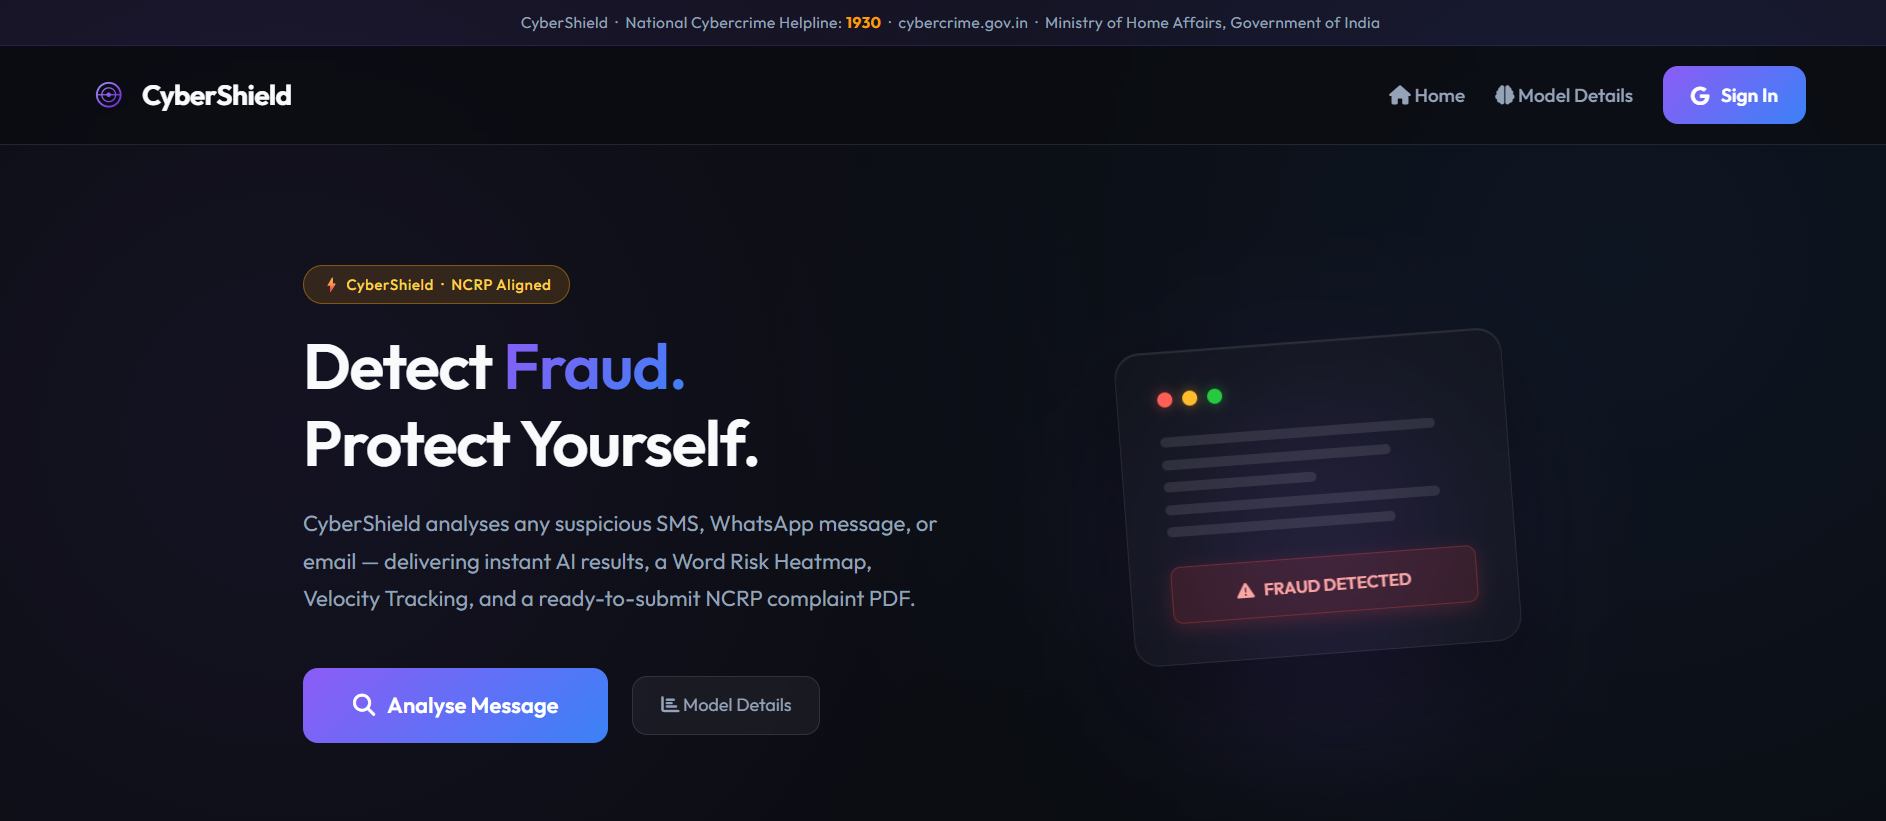
\includegraphics[width=0.82\textwidth,height=0.28\textheight,keepaspectratio]{report_file/landingpage.png}
    \caption{CyberShield citizen-facing landing page displaying the National Cybercrime Helpline (1930), link to cybercrime.gov.in, and Google OAuth authentication entry point.}
    \label{fig:landing}
\end{figure}

\begin{figure}[H]
    \centering
    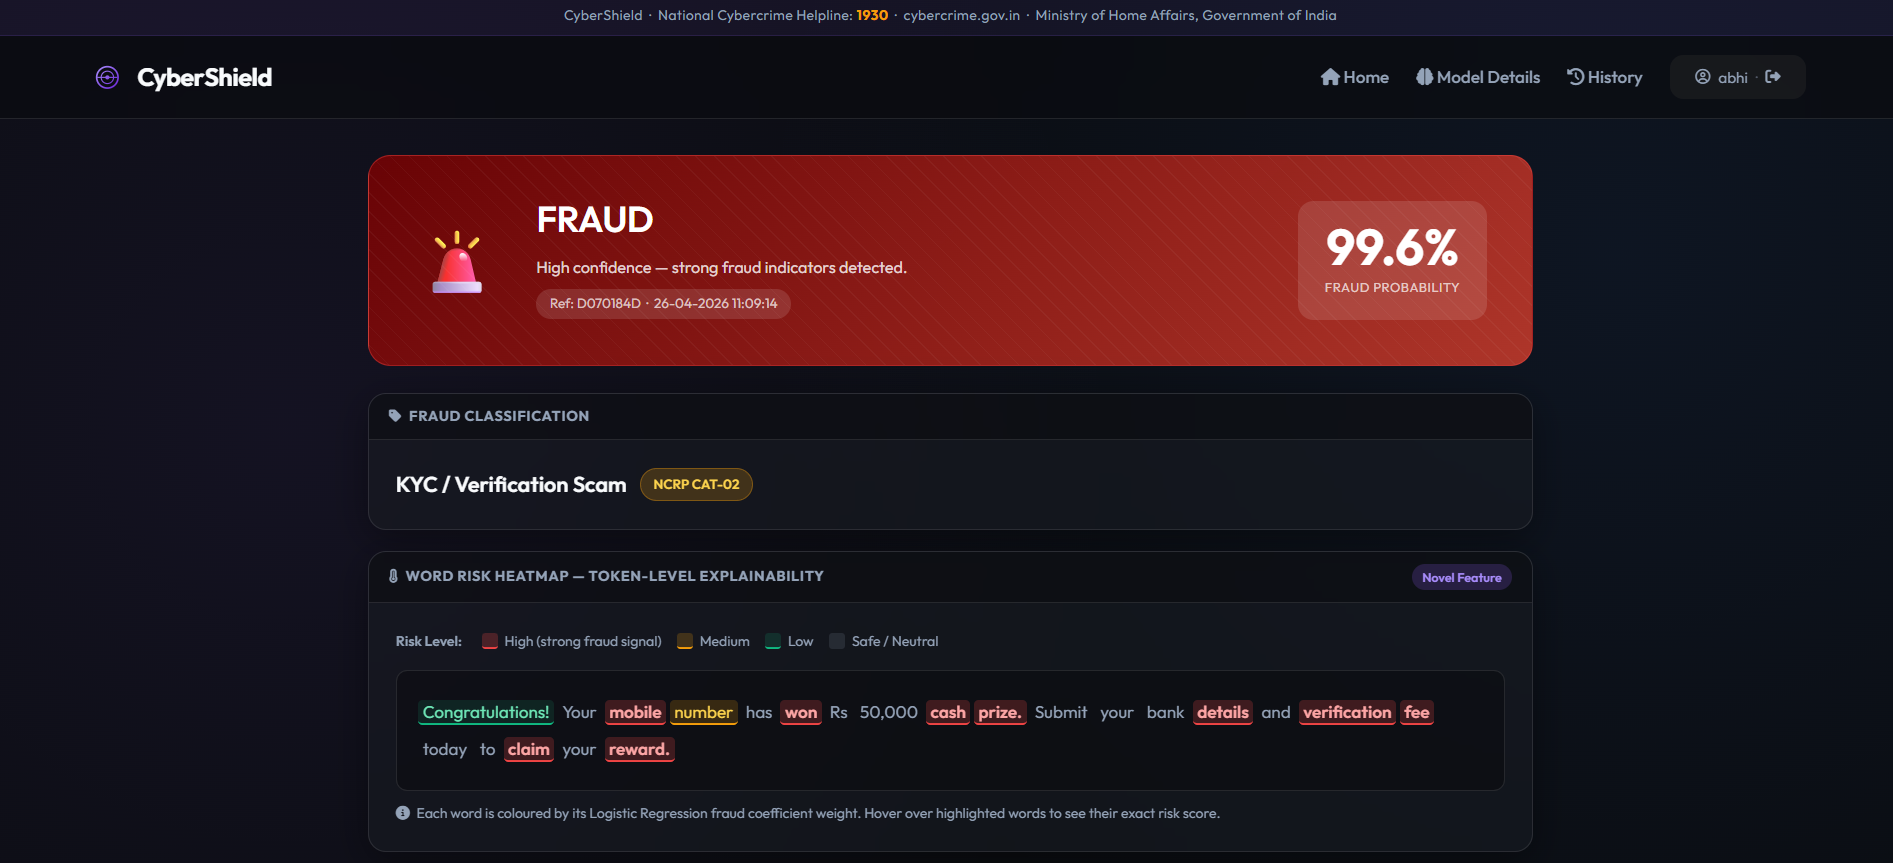
\includegraphics[width=0.82\textwidth,height=0.28\textheight,keepaspectratio]{report_file/result1.png}
    \caption{Analysis result for a high-confidence fraudulent message: risk badge, fraud probability, extracted artifacts, Word Risk Heatmap, and NCRP PDF generation button.}
    \label{fig:fraud_result}
\end{figure}

\begin{figure}[H]
    \centering
    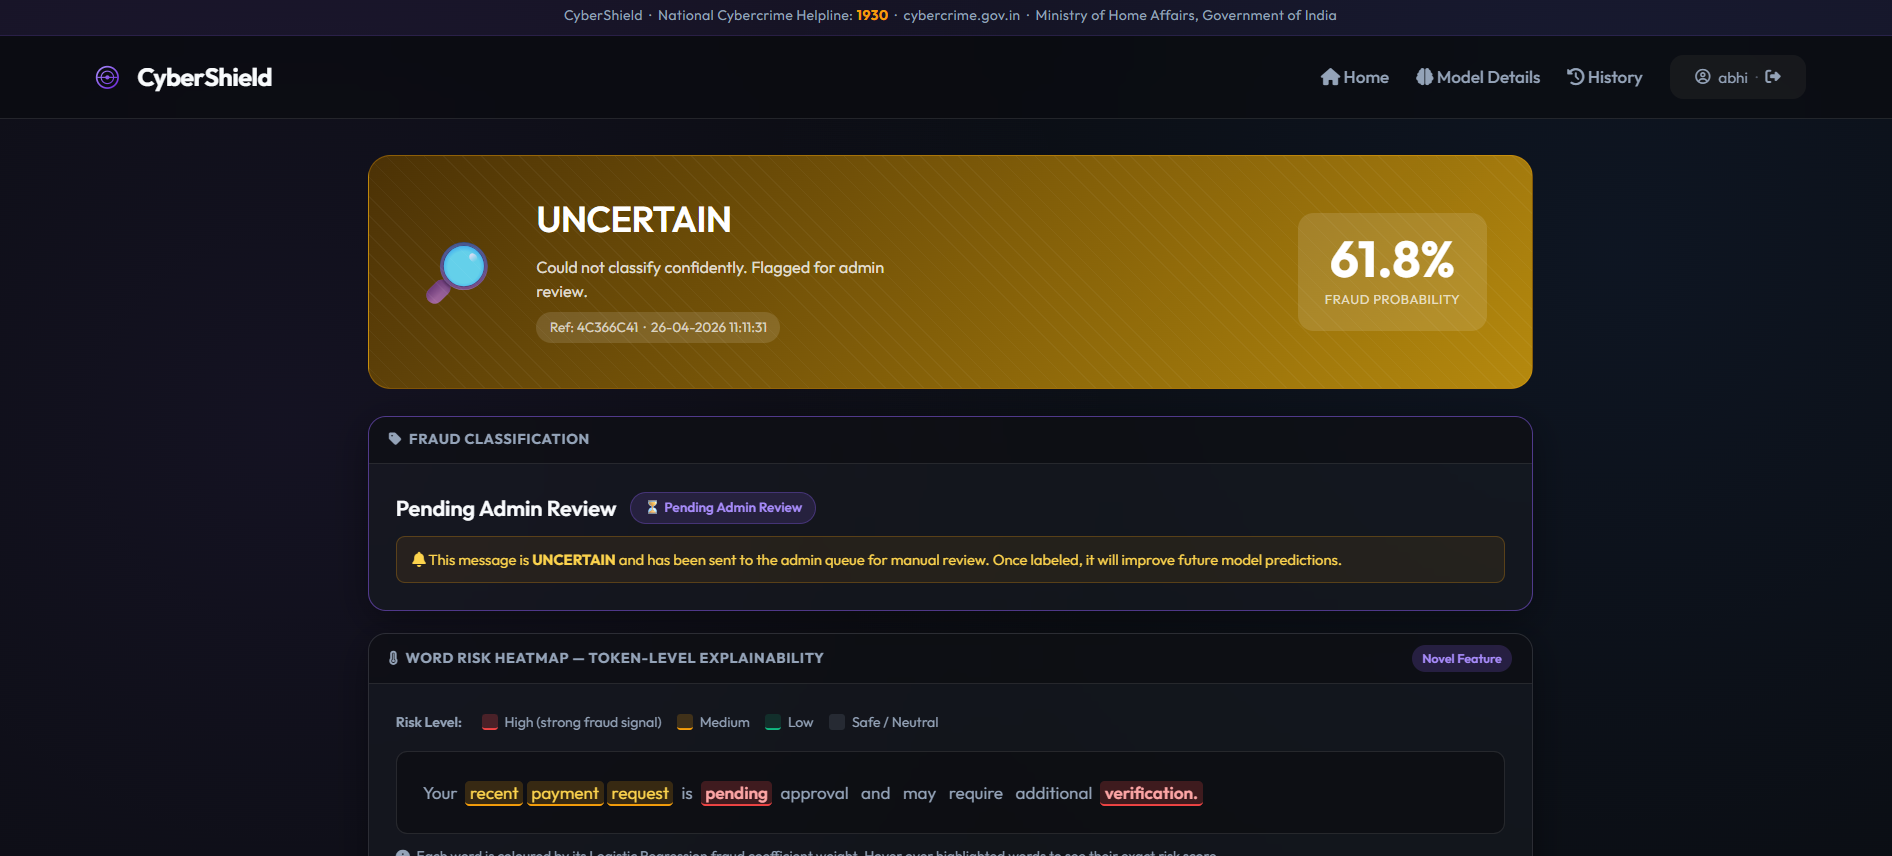
\includegraphics[width=0.82\textwidth,height=0.28\textheight,keepaspectratio]{report_file/uncertainResult.png}
    \caption{UNCERTAIN result ($P = 61.8\%$) routed to admin queue for HITL adjudication. Word Risk Heatmap highlights tokens \textit{recent}, \textit{payment}, \textit{request}, and \textit{verification} by LR coefficient weight.}
    \label{fig:uncertain}
\end{figure}

\begin{figure}[H]
    \centering
    \fbox{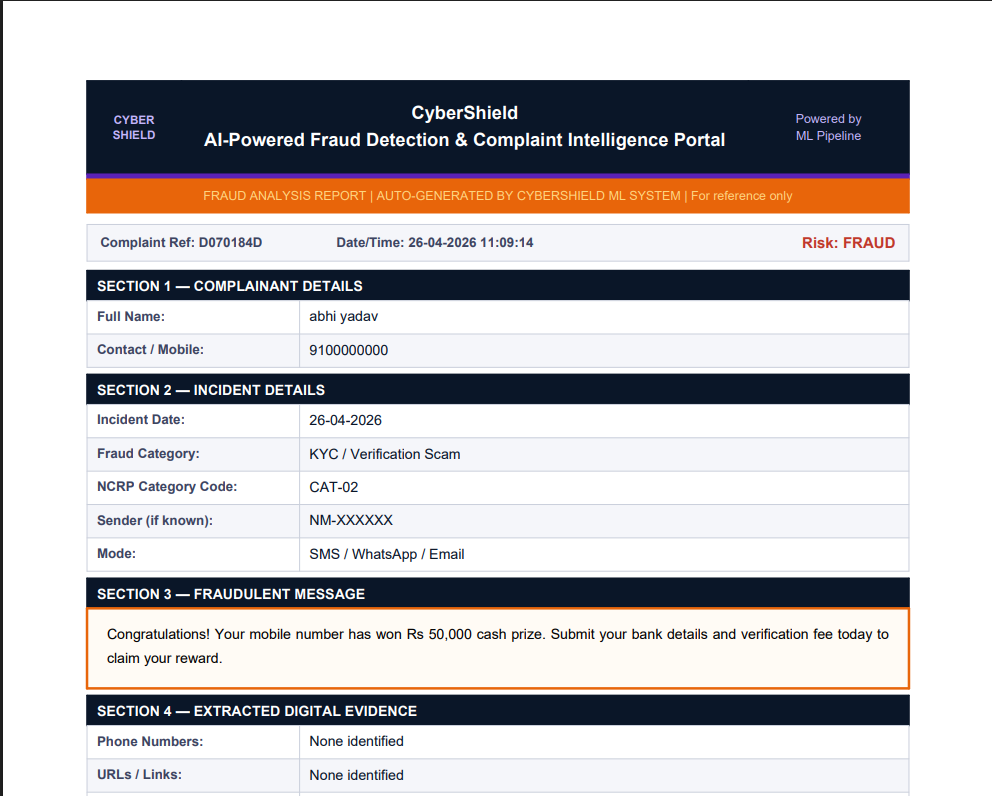
\includegraphics[width=0.80\textwidth,height=0.28\textheight,keepaspectratio]{report_file/pdfpart1.png}}
    \caption{Auto-generated NCRP-compliant PDF complaint document embedding complaint ID, timestamp, extracted IoCs, risk level, and fraud probability score.}
    \label{fig:pdf}
\end{figure}

\begin{figure}[H]
    \centering
    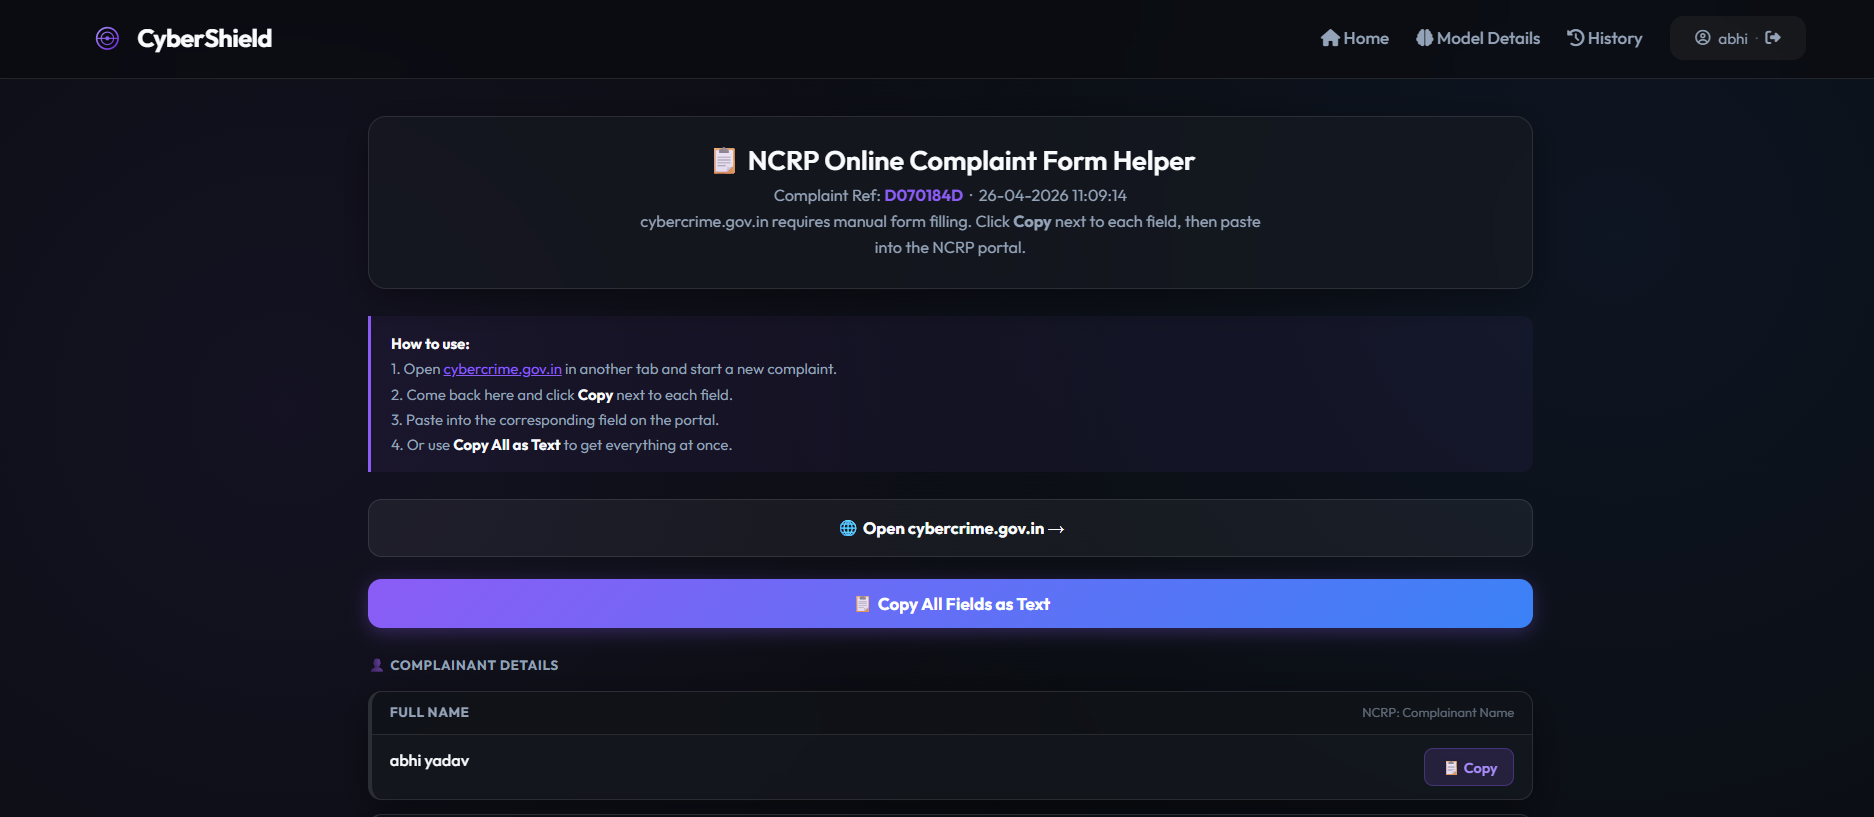
\includegraphics[width=0.82\textwidth,height=0.28\textheight,keepaspectratio]{report_file/NCRPhelper1.png}
    \caption{NCRP Online Form Helper pre-populating cybercrime.gov.in fields from the analysed message for single-click copy-paste submission.}
    \label{fig:ncrp_helper}
\end{figure}

\begin{figure}[H]
    \centering
    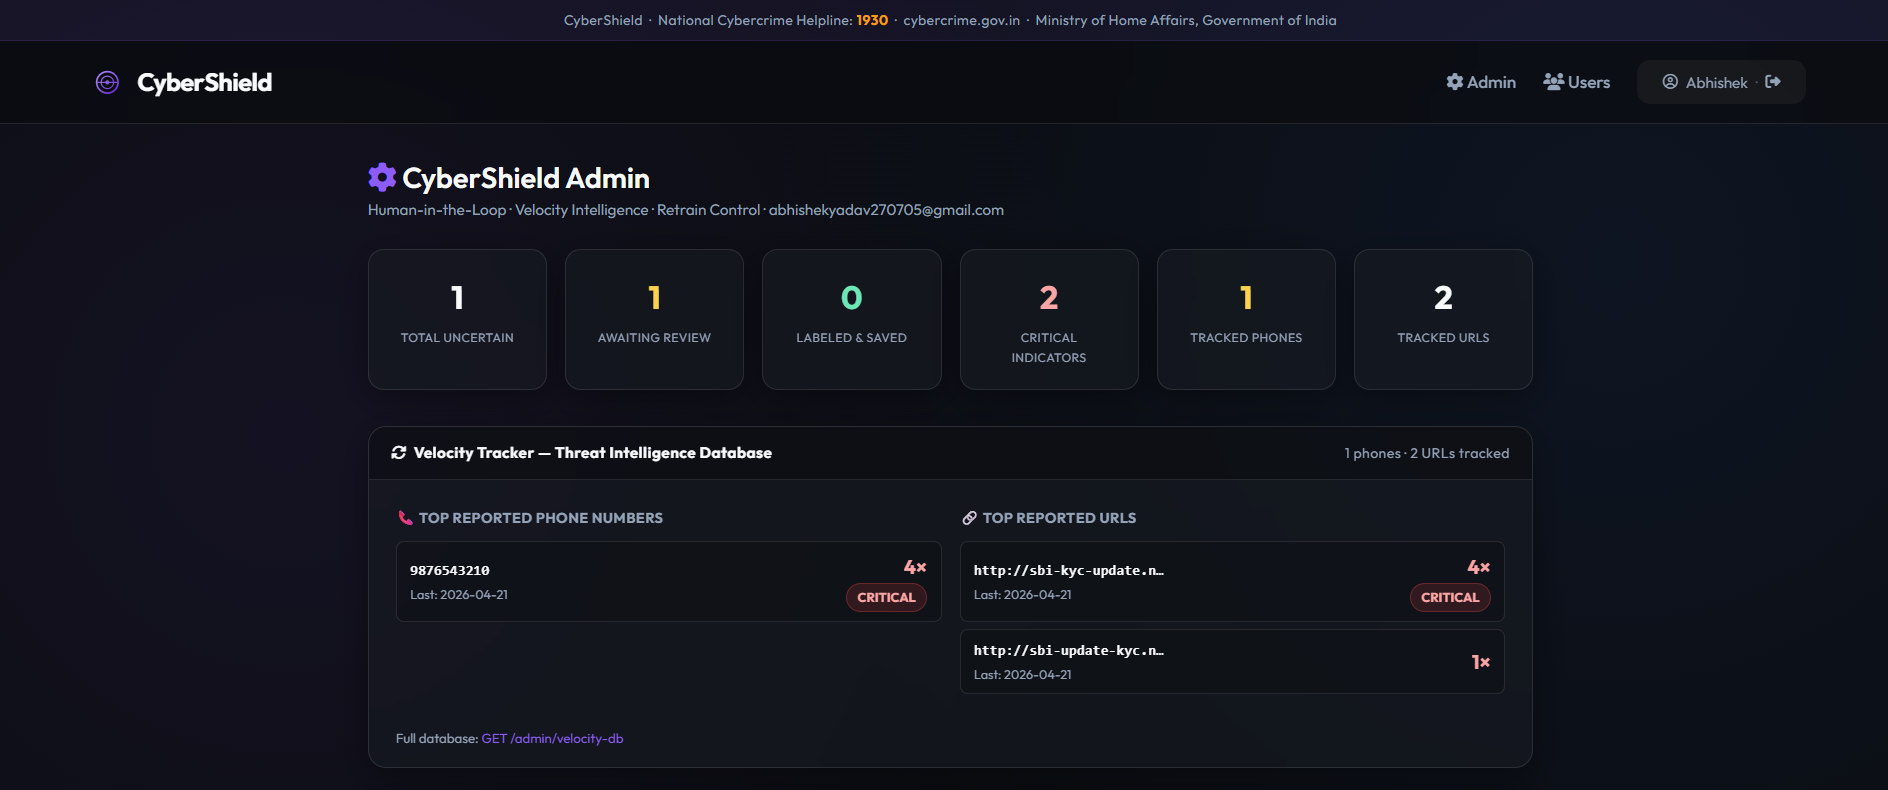
\includegraphics[width=0.82\textwidth,height=0.28\textheight,keepaspectratio]{report_file/admin.png}
    \caption{Admin Dashboard (OAuth-restricted) showing HITL queue and Velocity Intelligence DB. Phone 9876543210 and URL \texttt{http://sbi-kyc-update} are both CRITICAL after 4 independent submissions.}
    \label{fig:admin}
\end{figure}

\begin{figure}[H]
    \centering
    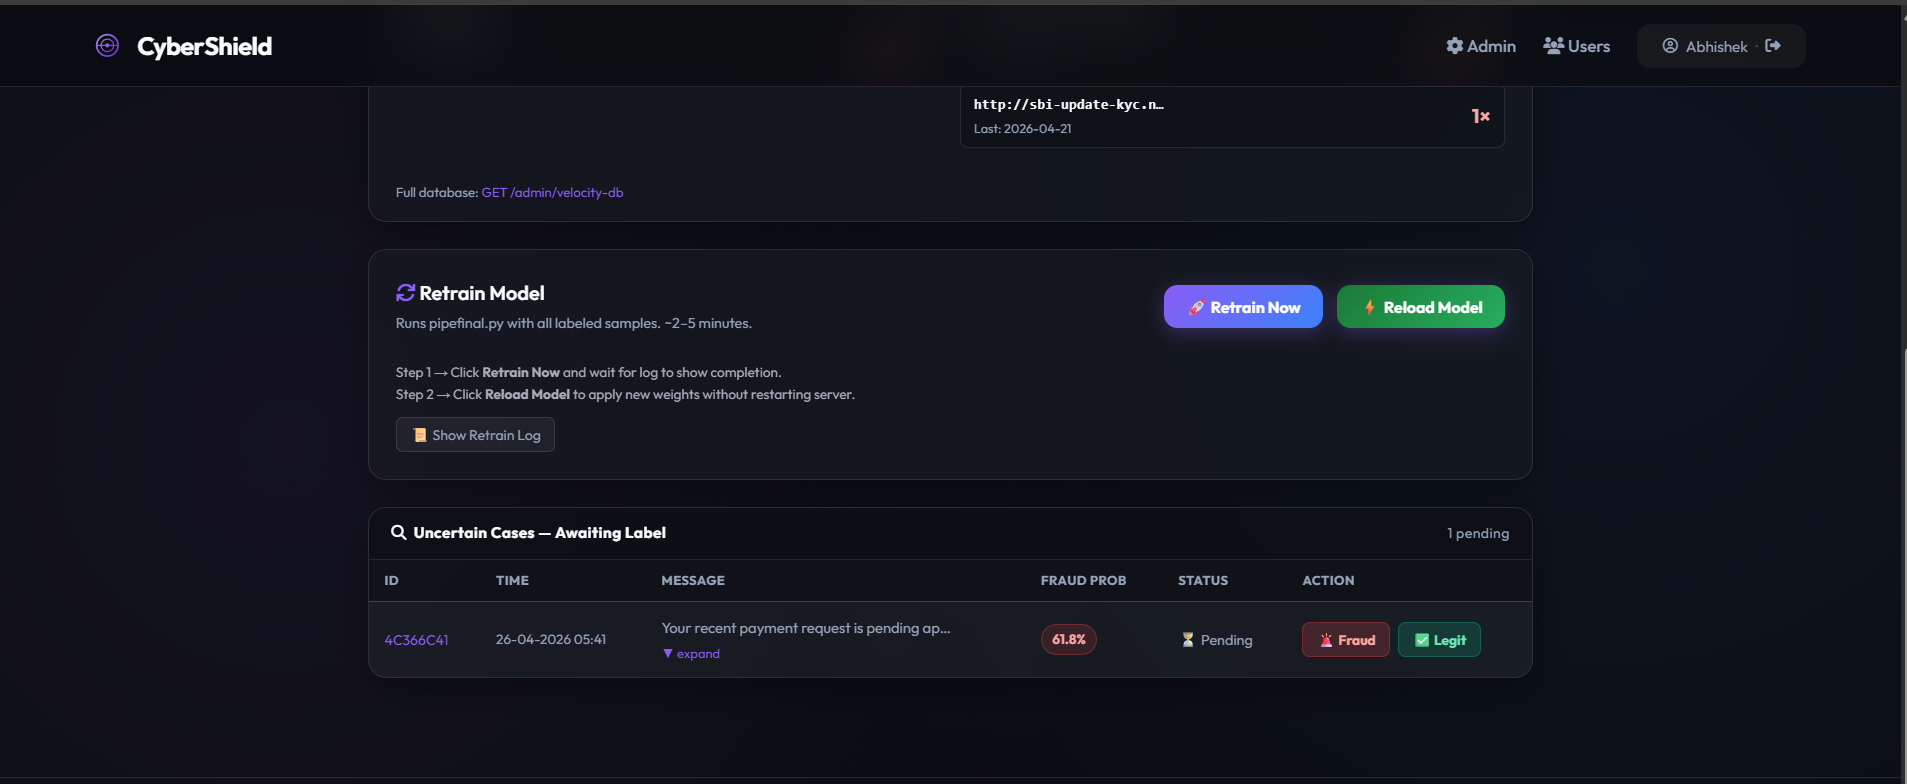
\includegraphics[width=0.82\textwidth,height=0.28\textheight,keepaspectratio]{report_file/admin1.png}
    \caption{Extended Admin Dashboard view showing comprehensive fraud investigation and systemic threat monitoring controls.}
    \label{fig:admin1}
\end{figure}

\begin{figure}[H]
    \centering
    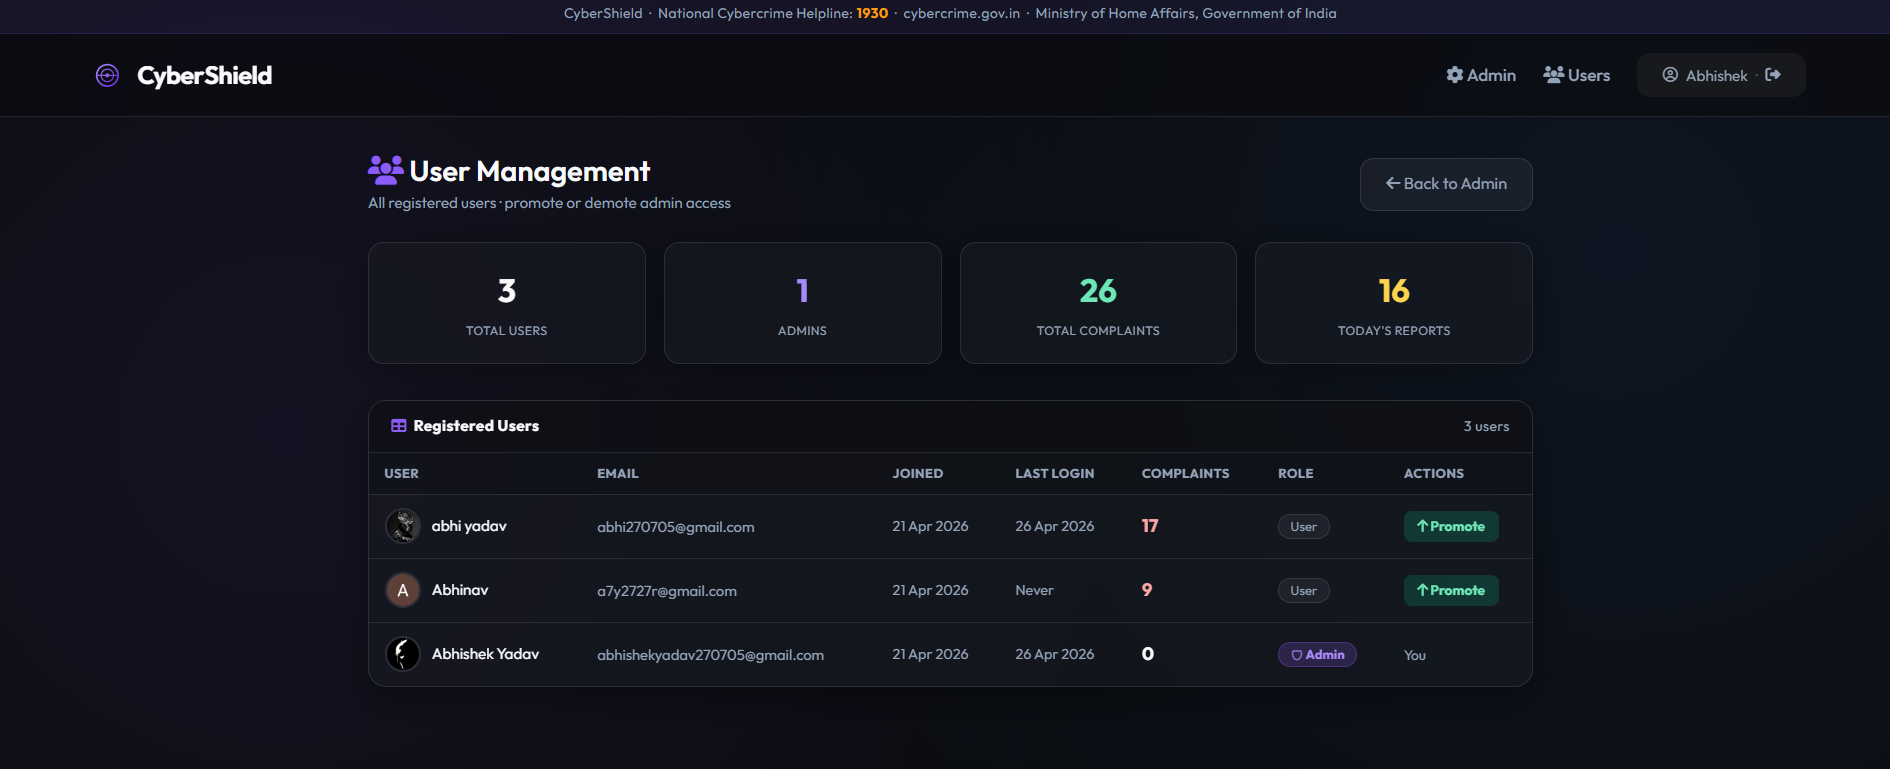
\includegraphics[width=0.82\textwidth,height=0.28\textheight,keepaspectratio]{report_file/admin2.png}
    \caption{User Management panel showing registered users, complaint counts, roles, and promote/demote administrative controls.}
    \label{fig:admin2}
\end{figure}

\section{Non-Functional Requirements Verification}

The five non-functional requirements defined in Section 3.5 were verified during system testing as follows.

\textbf{NFR1 (Inference Latency):} Real-time analysis of a 500-character SMS string - encompassing \texttt{vectorizer.transform()}, three \texttt{predict\_proba()} calls, RegEx artifact extraction, and velocity database update - consistently completed within 500 milliseconds under standard single-user load on the development hardware (Intel Core i5, 8 GB RAM). This threshold aligns with the UX research cited in Section 3.5 and was confirmed through repeated manual timing of the \texttt{/analyze} endpoint.

\textbf{NFR2 (Security and Authentication):} All administrative routes (\texttt{/admin}, \texttt{/admin/label}, \texttt{/admin/retrain}, \texttt{/admin/reload-model}, \texttt{/admin/velocity-db}) were verified to return HTTP 401 for unauthenticated requests and HTTP 403 for authenticated but non-whitelisted email addresses. The \texttt{@admin\_required} decorator was tested with both a whitelisted admin account and a standard citizen account to confirm correct access control behaviour.

\textbf{NFR3 (Idempotency of the Test Set):} The \texttt{split\_indices.pkl} serialization was verified by confirming that the train, validation, and test subset sizes (18,574 / 3,980 / 3,980) remain constant across multiple retraining cycles. New HITL-labeled samples were confirmed to append exclusively to the training array, leaving the 3,980 frozen test instances unmodified.

\textbf{NFR4 (Aesthetics and UX):} The citizen-facing interface, visible in Figures 6.4 through 6.8, implements a dark glassmorphic design with responsive layout. The interface was verified to render correctly on both desktop (1920$\times$1080) and mobile (Chrome mobile viewport, 390px width) screen sizes, confirming the responsive design requirement.

\textbf{NFR5 (Concurrent Access):} SQLAlchemy connection pooling with thread-local sessions was confirmed to handle concurrent \texttt{/analyze} submissions without raising database lock exceptions, replacing the raw SQLite3 WAL-mode approach used in the v3 architecture. Under the testing conditions described in Section 5.6.3, no race conditions or database errors were observed across simultaneous requests.

        \chapter{Conclusion}
        \section{Conclusion}
The literature review in Section 2.5 identified three critical gaps in contemporary fraud detection systems: the absence of uncertainty-aware classification architectures, a lack of end-to-end actionable intelligence pipelines for law enforcement, and vulnerability to rapid concept drift in adversarial threat vectors. In this project, we designed and evaluated \textbf{CyberShield}, an uncertainty-aware, Human-in-the-Loop fraud detection ecosystem specifically structured to resolve these deficiencies. CyberShield probabilistically structures risk across defined boundary strata: highly confident malicious patterns ($P \geq 0.90$) trigger automated generation of a pre-filled NCRP-compliant PDF for manual submission, ambiguous cases ($0.30 \leq P < 0.70$) are routed to a secure administrative queue for HITL adjudication \cite{holzinger2016interactive} and subsequent Hard Negative Mining, while safe messages ($P < 0.30$) are cleared without administrative overhead.

The mathematical ensemble of Logistic Regression, SVM, and Naive Bayes over a 25,000-feature TF-IDF matrix achieved \textbf{94.87\% test-set accuracy} and an \textbf{ROC-AUC of 0.9895} on a frozen partition of 3,980 adversarial examples. All five primary objectives defined in Section 1.4 were successfully realized: uncertainty-aware classification, HITL calibration, token-level explainability, velocity intelligence tracking, and automated NCRP adjudication. Critically, the novel \textit{False-Positive-Driven} Hard Negative Mining strategy --- which selectively mines the top 15\% highest-confidence False Positives and retrains using $w=2.0$ sample weights --- improved Fraud-class precision from 0.9508 to 0.9518 while holding recall perfectly stable at 0.9419. This validates the system's primary design constraint: blocking a legitimate citizen's message is operationally worse than missing a single spam, and the architecture was built to enforce this inequality mathematically. The wide UNCERTAIN band (0.30--0.70), which initially appears to sacrifice automation, is in fact the system's primary safety mechanism against catastrophic false negatives. By intertwining natural language semantic analysis with lexical URL/Phone Velocity Tracking, CyberShield demonstrates a pathway toward bridging the gap between raw AI predictions and actionable cyber-intelligence for law enforcement agencies. More broadly, acknowledging model uncertainty is not a weakness in deployed AI systems but a deliberate safety mechanism applicable to any high-stakes classification domain.

\section{Limitations of the Current System}
Despite the high mathematical efficacy, real-world deployment poses several limitations:
\begin{enumerate}
    \item \textbf{Multilingual Constraint:} The system relies on English and Romanglish (Hinglish) syntax. Regional scripts require external translation APIs or multilingual models (e.g., MuRIL).
    \item \textbf{Contextual Isolation:} Text is analyzed in isolation, lacking conversational memory required to detect multi-turn phishing engagements; future stateful session modeling is needed.
    \item \textbf{Adversarial Masking:} The character n-gram vectorizer is vulnerable to zero-width unicode insertion and homoglyph attacks; Unicode NFKC normalization and punycode decoding are required countermeasures.
    \item \textbf{Database Scalability:} SQLite's file-lock mechanism bottlenecks under high concurrency; migration to a Redis-based cache is recommended for scaling.
\end{enumerate}

\section{Future Scope}
The architectural modularity of CyberShield enables extensive scaling across three priority tiers:
\begin{itemize}
    \item \textbf{Near-Term --- NCRP Direct API Integration:} Establish a REST API connection with \texttt{cybercrime.gov.in} to auto-submit high-confidence cases ($P \geq 0.90$) as draft FIRs, replacing the current PDF-and-helper model.
    \item \textbf{Near-Term --- Browser Extension:} Package the inference endpoint as a browser extension for seamless in-context message analysis by citizens.
    \item \textbf{Medium-Term --- Multilingual Support:} Integrate translation pipelines or multilingual embeddings to process all regional Indian languages.
    \item \textbf{Medium-Term --- Transformer Inference:} Migrate to contextual embeddings via DistilBERT, provided the 500ms latency budget is consistently met on available infrastructure.
    \item \textbf{Long-Term --- Federated Learning:} Adapt the active-learning backend to federated schemas, enabling decentralized training across state cybercrime offices without exposing victim data.
    \item \textbf{Long-Term --- Multimodal Detection:} Expand ingestion to accept image screenshots (via OCR) and audio samples (via Speech-to-Text) to combat steganography and vishing threats.
\end{itemize}

        
        \bibliography{report}
	\bibliographystyle{plain}
        
	
	
	
	
\end{document}
